\documentclass[11pt,a4paper,oneside]{report}

% --- Language & Encoding ---
\usepackage[utf8]{inputenc}
\usepackage[T1]{fontenc}

% --- Page Geometry ---
\usepackage[top=1in, bottom=1in, left=1in, right=1in]{geometry}

% --- Colors ---
\usepackage{xcolor}
\definecolor{RguktMaroon}{HTML}{800000}
\definecolor{RguktGold}{HTML}{FFD700}
\definecolor{Charcoal}{HTML}{111827}
\definecolor{LightGrey}{HTML}{F9FAFB}
\definecolor{BorderGrey}{HTML}{E2E8F0}
\definecolor{CodeGreen}{HTML}{008000}
\definecolor{CodeBlue}{HTML}{0000FF}
\definecolor{CodePurple}{HTML}{800080}

% --- Typography ---
\usepackage{amsmath}
\usepackage{microtype}
\usepackage{helvet}
\renewcommand{\familydefault}{\sfdefault} % Modern sans-serif look

% --- Navigation & Hyperlinks ---
\usepackage[pdftex]{graphicx}
\usepackage{float}
\usepackage{caption}
\usepackage{subcaption}
\usepackage[hidelinks]{hyperref}
\usepackage{bookmark}

% --- Tables ---
\usepackage{booktabs}
\usepackage{tabularx}
\usepackage{longtable}

% --- Code Formatting ---
\usepackage{listings}
\lstset{
    backgroundcolor=\color{LightGrey},
    basicstyle=\ttfamily\small\color{Charcoal},
    breakatwhitespace=false,
    breaklines=true,
    captionpos=b,
    commentstyle=\color{CodeGreen},
    keywordstyle=\color{CodeBlue}\bfseries,
    stringstyle=\color{CodePurple},
    frame=single,
    rulecolor=\color{BorderGrey},
    keepspaces=true,
    numbers=left,
    numberstyle=\tiny\color{gray},
    numbersep=5pt,
    showspaces=false,
    showstringspaces=false,
    showtabs=false,
    tabsize=2
}

\lstdefinelanguage{json}{
    basicstyle=\ttfamily\small\color{Charcoal},
    backgroundcolor=\color{LightGrey},
    numbers=left,
    numberstyle=\tiny\color{gray},
    showstringspaces=false,
    breaklines=true,
    frame=single,
    rulecolor=\color{BorderGrey},
    string=[s]{"}{"},
    stringstyle=\color{CodePurple},
    comment=[l]{//},
    morecomment=[s]{/*}{*/},
    commentstyle=\color{CodeGreen},
    literate=
     *{0}{{{\color{CodeBlue}0}}}{1}
      {1}{{{\color{CodeBlue}1}}}{1}
      {2}{{{\color{CodeBlue}2}}}{1}
      {3}{{{\color{CodeBlue}3}}}{1}
      {4}{{{\color{CodeBlue}4}}}{1}
      {5}{{{\color{CodeBlue}5}}}{1}
      {6}{{{\color{CodeBlue}6}}}{1}
      {7}{{{\color{CodeBlue}7}}}{1}
      {8}{{{\color{CodeBlue}8}}}{1}
      {9}{{{\color{CodeBlue}9}}}{1}
      {:}{{{\color{RguktMaroon}{:}}}}{1}
      {,}{{{\color{RguktMaroon}{,}}}}{1}
      {\{}{{{\color{Charcoal}{\{}}}}{1}
      {\}}{{{\color{Charcoal}{\}}}}}{1}
      {[}{{{\color{Charcoal}{[}}}}{1}
      {]}{{{\color{Charcoal}{]}}}}{1},
}

% --- TikZ for Diagrams ---
\usepackage{tikz}
\usetikzlibrary{shapes.geometric, arrows, positioning, fit, calc, backgrounds}
\tikzstyle{block} = [rectangle, draw=RguktMaroon, fill=white, text=Charcoal, minimum width=3.5cm, minimum height=1.2cm, text centered, rounded corners, line width=1.2pt, align=center]
\tikzstyle{cloud} = [ellipse, draw=RguktMaroon, fill=white, text=Charcoal, minimum width=2.5cm, minimum height=1cm, text centered, line width=1.2pt, align=center]
\tikzstyle{arrow} = [thick,->,>=stealth,color=RguktMaroon,line width=1.1pt]
\tikzstyle{line} = [thick,-,color=RguktMaroon,line width=1.1pt]

% --- Headers & Footers ---
\usepackage{fancyhdr}
\pagestyle{fancy}
\fancyhf{}
\fancyhead[L]{\textcolor{RguktMaroon}{\textbf{RGUKT Connect}}}
\fancyhead[R]{\textcolor{gray}{\leftmark}}
\fancyfoot[C]{\thepage}
\renewcommand{\headrulewidth}{0.5pt}
\renewcommand{\footrulewidth}{0.0pt}

% --- Section Spacing & Titles ---
\usepackage{titlesec}
\titleformat{\chapter}[display]
  {\normalfont\huge\bfseries\color{RguktMaroon}}
  {\chaptername\ \thechapter}{20pt}{\Huge}
\titleformat{\section}
  {\normalfont\Large\bfseries\color{RguktMaroon}}{\thesection}{1em}{}
\titleformat{\subsection}
  {\normalfont\large\bfseries\color{RguktMaroon}}{\thesubsection}{1em}{}

% --- Bibliography Settings ---
\usepackage{cite}

\begin{document}

% ==========================================
% COVER PAGE
% ==========================================
\begin{titlepage}
    \centering
    \vspace*{1.5cm}
    
    {\Huge \bfseries \color{RguktMaroon} RGUKT Connect} \\[0.5cm]
    {\Large \bfseries \color{Charcoal} Technical and Product Documentation} \\[0.8cm]
    
    \vspace{1.5cm}
    
    % Professional Vector Accent Box
    
\begin{tikzpicture}
        \draw[line width=3pt, color=RguktMaroon] (0,0) -- (12,0);
        \draw[line width=1pt, color=RguktGold] (0,-0.2) -- (12,-0.2);
    \end{tikzpicture}
    
    \vspace{1.5cm}
    
    \begin{minipage}{0.8\textwidth}
        \centering
        \large \color{Charcoal}
        A secure, dedicated professional networking platform bridging alumni and students of Rajiv Gandhi University of Knowledge Technologies.
    \end{minipage}
    
    \vspace{2.5cm}
    
    \large
    \textbf{Project Context:} Professional Peer Networking, Referrals, and Mentorship \\
    \textbf{Target Audience:} Software Engineers, Recruiters, Collaborators, and Alumni \\
    
    \vfill
    
    
\begin{tikzpicture}
        \draw[line width=1pt, color=RguktGold] (0,0) -- (12,0);
        \draw[line width=3pt, color=RguktMaroon] (0,-0.2) -- (12,-0.2);
    \end{tikzpicture}
    
    \vspace{0.8cm}
    
    {\large \color{Charcoal} Version 2.0.0 | \today}
\end{titlepage}

% ==========================================
% EXECUTIVE SUMMARY (Before Chapters)
% ==========================================
\chapter*{Executive Summary}
\addcontentsline{toc}{chapter}{Executive Summary}

RGUKT Connect is an enterprise-grade professional networking and mentorship platform designed exclusively for the community of the Rajiv Gandhi University of Knowledge Technologies (RGUKT). Built to establish a secure, verified digital bridge between current university students and alumni working in the industry, the platform facilitates direct career guidance, verified job referrals, and real-time collaboration.

\section*{Key Capabilities}
\begin{itemize}
    \item \textbf{Secure Verification:} Restricts enrollment to authorized university members through a dual-step identity verification requiring a valid `@rgukt.ac.in` domain and individual student ID numbers validated via automated One-Time Passwords (OTP).
    \item \textbf{Verified Professional Portfolios:} Offers comprehensive profiles containing detailed academic histories, verified work experiences, project source linkages (GitHub/LinkedIn), and academic branches.
    \item \textbf{Mentorship and Alumni Directory:} Provides a searchable directory of the RGUKT network, allowing students to easily discover and reach out to seniors who possess active careers in specific organizations.
    \item \textbf{Direct Referrals \& Job Board:} Enables verified alumni and administrators to publish career opportunities and offer direct referrals, skipping the generic application process.
    \item \textbf{Real-Time Messaging:} Employs a STOMP-based WebSocket communication layer to enable instant, persistent messaging between connected members.
\end{itemize}

\section*{Technical Overview}
RGUKT Connect features a modern split-architecture. The backend is powered by Java 21, Spring Boot 3/4, Spring Security, Hibernate ORM, and a PostgreSQL database. It offloads binary assets (such as profile pictures and post media) directly to Amazon S3. The frontend is built as a highly responsive single-page application using React 19, Vite, Tailwind CSS 4.0, and Axios. Real-time notifications and message deliveries are bridged using a STOMP messaging broker over WebSockets. Deployment is optimized using containerized Docker environments managed by a Jenkins automation pipeline and orchestrated inside a Kubernetes cluster.

% ==========================================
% TOC, FIGURES, TABLES
% ==========================================
\tableofcontents
\listoffigures
\listoftables

% ==========================================
% CHAPTERS INCLUSION
% ==========================================
\chapter{Introduction}
\label{ch:introduction}

Rajiv Gandhi University of Knowledge Technologies (RGUKT) is a premier state university in India, established with the mission of providing high-quality technical education to rural youth. Operating across multiple campuses (including Nuzvid, RK Valley, Srikakulam, and Ongole), RGUKT has produced thousands of engineering graduates who are now employed in major global technology companies, research centers, and public service organizations. 

Despite this large, talented, and highly dispersed alumni pool, there has historically been a significant digital gap between current students on campus and alumni in the industry. Communication has remained fragmented across unofficial channels, such as local WhatsApp groups, Facebook pages, and Telegram channels. These unofficial channels fail to provide a structured environment for professional networking, persistent knowledge sharing, or direct, secure job referrals.

\section{Project Motivation}
The motivation for building \textbf{RGUKT Connect} stems from three primary requirements:
\begin{enumerate}
    \item \textbf{Institutional Trust Validation:} LinkedIn and other global professional networks do not verify academic records in a trustless manner. Anyone can claim an affiliation with RGUKT, which introduces a potential verification gap. There is an urgent need for a network limited strictly to verified RGUKT members.
    \item \textbf{Direct Alumni Referral Channels:} Current recruitment processes are heavily congested. Standard online applications often fall into resume blackholes. Direct referrals from active employees inside companies offer the highest conversion rates for students. A platform that directly links students to alumni for referrals dramatically improves placement rates.
    \item \textbf{Persistent Mentorship:} Students require structured feedback on resumes, projects, and interview preparation. Connecting them with alumni in matching engineering roles provides direct, high-value industry mentorship.
\end{enumerate}

\section{System Objectives}
The primary objectives of the RGUKT Connect platform are to:
\begin{itemize}
    \item Establish a secure platform restricted to verified students and alumni by verifying their university-issued email domain (`@rgukt.ac.in`) and 7-character registration ID.
    \item Provide an interactive community feed where users can share professional news, code snippets, and post media.
    \item Implement a searchable directory to locate alumni by branch, batch, company, and role.
    \item Build a real-time messaging gateway to allow instant communication between connected users without sharing personal phone numbers or email addresses.
    \item Maintain a dedicated job board for verified alumni to post active job opportunities and internship openings.
\end{itemize}

\section{Document Scope}
This document serves as the complete technical and product blueprint for RGUKT Connect. It provides a comprehensive analysis of the system architecture, product characteristics, technical stack, database designs, authentication mechanisms, deployment methodologies, and operational workflows. It is intended for software engineers, deployment specialists, recruiters, and prospective collaborators seeking a deep architectural understanding of the platform.

\chapter{Problem Statement}
\label{ch:problem_statement}

In the professional networking landscape, students and graduates of Rajiv Gandhi University of Knowledge Technologies (RGUKT) face unique structural hurdles. To understand the need for a specialized university network, we must analyze the existing communication deficits and operational challenges.

\section{Analysis of Current Communication Deficits}
Currently, the RGUKT community relies on general-purpose social networks (such as LinkedIn, Facebook, and Twitter) or private messaging channels (such as WhatsApp and Telegram) to manage alumni-student communication. These general-purpose channels exhibit major limitations:
\begin{itemize}
    \item \textbf{Fragmentation:} Unofficial messaging groups are restricted by size limits (e.g., WhatsApp group limits) and split by batches or branches. This splits the network into isolated clusters, preventing unified outreach.
    \item \textbf{High Signal-to-Noise Ratio:} General-purpose groups are often saturated with non-professional discussions, meme sharing, and administrative announcements, making it difficult for users to isolate high-value career discussions or referral posts.
    \item \textbf{Searchability Issues:} Messaging applications do not structure profile data. A student cannot run a query to find a senior who graduated in 2021 with a CSE degree and currently works as a cloud engineer at a specific target company.
\end{itemize}

\section{The Verification Gap and Trust Deficit}
A critical vulnerability in public networking websites is the absence of verification controls for institutional associations:
\begin{itemize}
    \item \textbf{Affiliation Spoofing:} Anyone can create a public profile on LinkedIn and assert that they are a student or graduate of RGUKT. This lack of validation introduces a security vulnerability, opening the door for phishing and social engineering.
    \item \textbf{Spamming Alumni:} Because public networks are open, alumni are often flooded with generic connection requests and cold messages from strangers outside their university circle. This causes network fatigue, causing alumni to ignore legitimate student inquiries.
\end{itemize}

\section{The Job Referral Bottleneck}
Getting job interviews through standard resume portal applications has become increasingly difficult due to automated Applicant Tracking System (ATS) filtering. Direct referrals from employees bypass these filters and guarantee manual review. However, the path to a referral is blocked:
\begin{itemize}
    \item \textbf{Lack of Direct Context:} Cold emailing or cold messaging alumni on LinkedIn without a shared context is often ignored.
    \item \textbf{Friction in Posting:} Alumni who want to help their juniors by referring them for active openings in their companies have no central university dashboard to post these listings. They must post on personal feeds, where reach is limited.
\end{itemize}

\section{The Proposed Solution: RGUKT Connect}
RGUKT Connect resolves these challenges by establishing a closed-loop, verified network restricted strictly to the RGUKT ecosystem. By verifying accounts through university email domains (`@rgukt.ac.in`) and university-issued student registration IDs, the platform guarantees that every user is authentic. It integrates a structured directory, direct job and referral postings, a social feed, and real-time private messaging in a single, secure space.

\chapter{Product Overview}
\label{ch:product_overview}

RGUKT Connect is designed as a secure, specialized, and real-time professional ecosystem. This chapter details the core product definition, its target user groups, boundaries, and the general user journey.

\section{Target User Roles}
The platform is designed around three main user groups within the university community:
\begin{enumerate}
    \item \textbf{Students (Current Undergraduates):} Users seeking career guidance, mentorship, project reviews, and direct job or internship referrals. They use the platform to search for alumni, build professional profiles, participate in discussions, and apply for listings.
    \item \textbf{Alumni (Graduated Professionals):} Users who are currently employed in the industry or pursuing advanced degrees. They act as mentors, write posts sharing industry trends, publish job openings from their employers, and offer direct referrals.
    \item \textbf{Administrators (Platform Managers):} Users responsible for managing the platform. They can delete posts, manage jobs, check system health, and oversee user activity.
\end{enumerate}

\section{Platform Boundaries}
To preserve security and institutional focus, the platform maintains strict operational boundaries:
\begin{itemize}
    \item \textbf{Closed Registration:} Only users with emails ending in `@rgukt.ac.in` and 7-character registration numbers can sign up. External registrations are rejected.
    \item \textbf{Verification Loop:} System interaction is blocked until the registration email is verified using a 6-digit OTP delivered via SMTP.
    \item \textbf{Connection-Based Interaction:} To prevent spam, private messaging is restricted. A student can only initiate a direct chat with an alumnus or other student once they send a connection request and the recipient accepts it.
\end{itemize}

\section{User Journey \& Flow}
The user journey is divided into authentication, discovery, and engagement. When a user first opens the web application, the root route checks the LocalStorage session token. If the token is missing or expired, the user is redirected to the public Landing page, where they can choose to log in or register. Once authenticated, they enter the main platform containing the Home Feed, Network Directory, Jobs Board, Chat client, and Profile dashboard.

Figure~\ref{fig:user_flow} shows the complete user journey flowchart.

\begin{figure}[H]
    \centering
    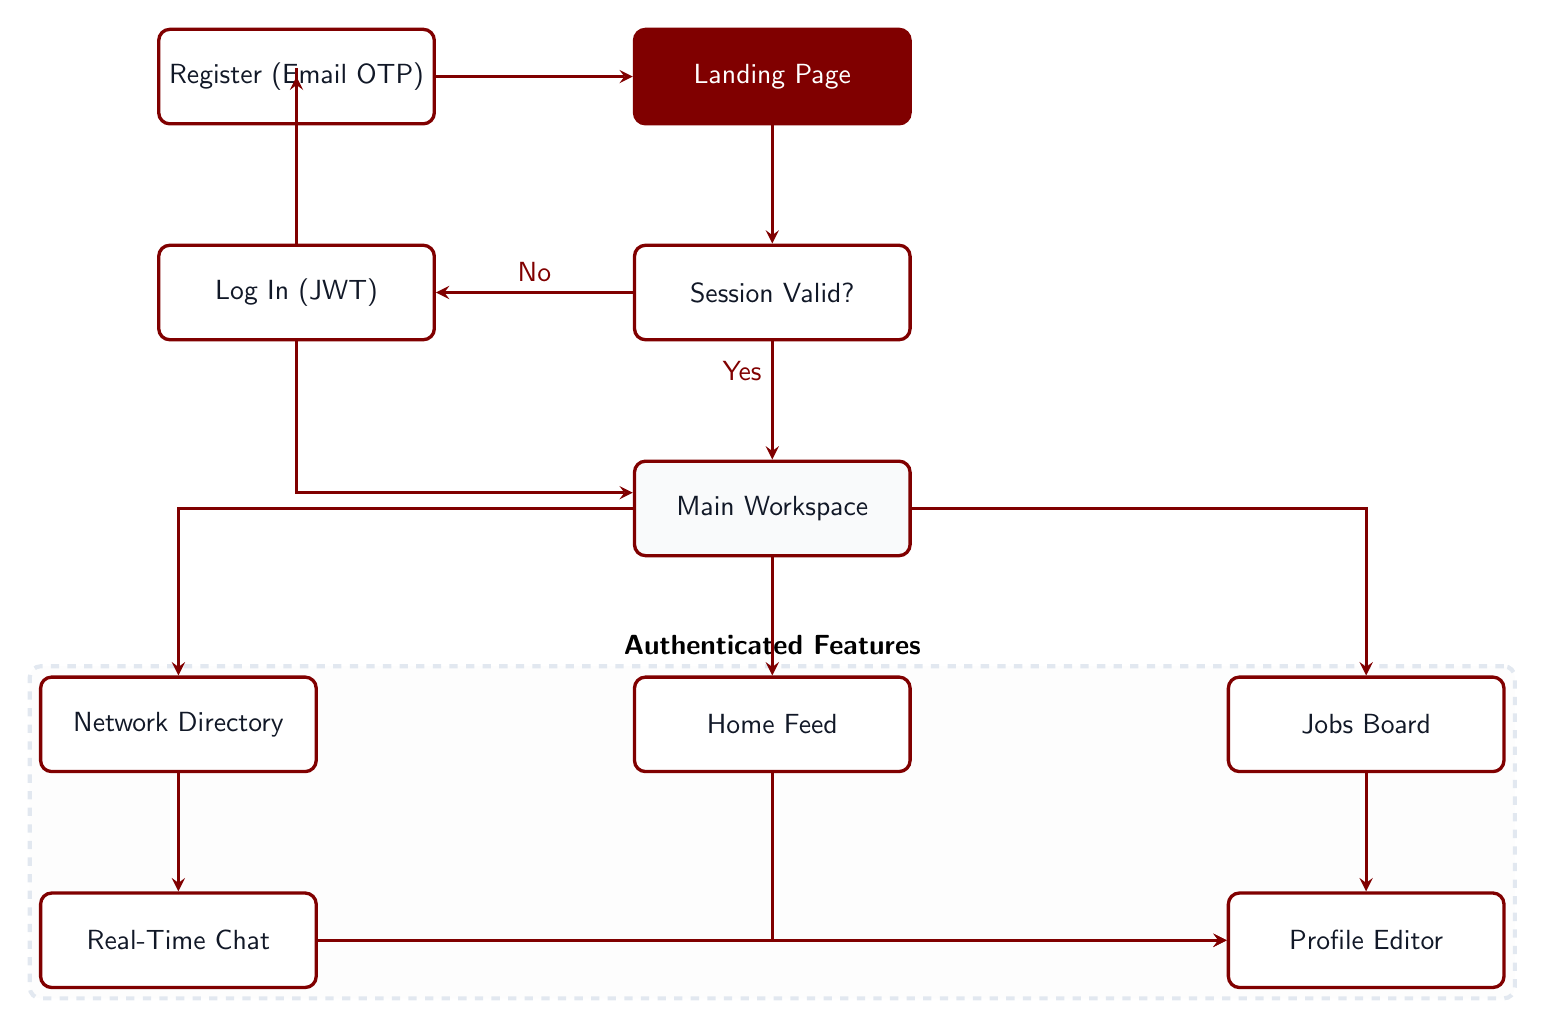
\begin{tikzpicture}[node distance=2cm, auto]
        % Define block styles locally if needed
        \node [block, fill=RguktMaroon, text=white] (landing) {Landing Page};
        \node [block, below=1.5cm of landing] (authCheck) {Session Valid?};
        
        \node [block, left=2.5cm of authCheck] (login) {Log In (JWT)};
        \node [block, left=2.5cm of landing] (register) {Register (Email OTP)};
        
        \node [block, below=1.5cm of authCheck, fill=LightGrey] (workspace) {Main Workspace};
        
        \node [block, below=1.5cm of workspace] (feed) {Home Feed};
        \node [block, left=4cm of feed] (network) {Network Directory};
        \node [block, right=4cm of feed] (jobs) {Jobs Board};
        \node [block, below=1.5cm of network] (chat) {Real-Time Chat};
        \node [block, below=1.5cm of jobs] (profile) {Profile Editor};

        % Connect nodes
        \draw [arrow] (landing) -- (authCheck);
        \draw [arrow] (authCheck) -- node [near start, left] {Yes} (workspace);
        \draw [arrow] (authCheck) -- node [above] {No} (login);
        \draw [arrow] (login) |- (register);
        \draw [arrow] (register) -- (landing);
        \draw [arrow] (login) |- ($(workspace.west) + (0,0.2)$);
        
        \draw [arrow] (workspace) -- (feed);
        \draw [arrow] (workspace) -| (network);
        \draw [arrow] (workspace) -| (jobs);
        
        \draw [arrow] (network) -- (chat);
        \draw [arrow] (jobs) -- (profile);
        \draw [arrow] (feed) |- (profile);
        \draw [arrow] (chat) -- (profile);
        
        % Background shading
        \begin{scope}[on background layer]
            \node[draw=BorderGrey, dashed, line width=1.5pt, fill=LightGrey!40, rounded corners, fit=(feed) (network) (jobs) (chat) (profile), label=above:\textbf{Authenticated Features}] (box) {};
        \end{scope}
    \end{tikzpicture}
    \caption{RGUKT Connect User Journey and Platform Navigation Flow}
    \label{fig:user_flow}
\end{figure}

\chapter{Features}
\label{ch:features}

This chapter details the functional capabilities of the RGUKT Connect platform, including validation logic, storage configurations, and network constraints.

\section{Identity Verification \& OTP Lifecycle}
Account security begins during registration and password recovery.
\begin{itemize}
    \item \textbf{Registration Verification:} Users enter their name, university email, and student ID. The system validates that the email domain matches `@rgukt.ac.in` and the ID is exactly 7 characters. It generates a 6-digit OTP, stores it in an in-memory `ConcurrentHashMap` with a 5-minute expiry, and sends it via SMTP.
    \item \textbf{Password Recovery:} The recovery process uses a similar workflow. The system verifies the user exists, generates an OTP, and requires its submission alongside a new password.
    \item \textbf{Testing Shortcut:} To streamline automated testing and development, emails starting with the prefix `test` bypass SMTP sending. The system hardcodes the OTP to `123456`.
\end{itemize}

\section{Alumni Directory \& Connection Management}
Discovering other members and establishing contact uses a directory and a connection workflow:
\begin{itemize}
    \item \textbf{Directory Search:} Users can search the global registry, which lists name, batch, branch, profile picture, and current employment role. The directory automatically excludes the current user.
    \item \textbf{Relationship Matrix:} Connections use a state machine with the states:
    \begin{itemize}
        \item \texttt{NOT\_CONNECTED}: No relationship exists. Users see a "Connect" option.
        \item \texttt{PENDING\_SENT}: The current user sent a request. They see a "Pending" option.
        \item \texttt{PENDING\_RECEIVED}: The current user received a request. They see "Accept" and "Reject" options.
        \item \texttt{ACCEPTED}: The connection is established. Users can send private messages.
    \end{itemize}
    \item \textbf{Action Handling:} Rejecting or cancelling a request deletes the database row. Accepting updates the status to \texttt{ACCEPTED} and triggers a real-time notification to the sender.
\end{itemize}

\section{Real-Time STOMP Messaging}
Private messaging uses WebSockets to support real-time delivery:
\begin{itemize}
    \item \textbf{STOMP Protocol:} The client connects using a STOMP client over WebSockets (`ws://<host>/ws-chat/websocket`). The connection handshake includes a JWT token in the `Authorization` header, which is validated by a custom WebSocket channel interceptor.
    \item \textbf{Topic Subscriptions:} Users subscribe to `/user/queue/messages` for incoming messages. Sent messages are posted to `/api/chat/send` and saved to PostgreSQL.
    \item \textbf{Delivery Indicators:} The UI displays unread counts. If a user is not currently viewing the active chat, the app increments the unread count and plays a notification sound.
\end{itemize}

\section{Opportunities Board \& Job Referrals}
To streamline employment opportunities, the platform provides a dedicated Job Board:
\begin{itemize}
    \item \textbf{Role Restrictions:} Only users with the role `ALUMNI` or `ADMIN` can post jobs or mark posts as `referral`. If a student attempts to post, the system returns a validation error.
    \item \textbf{Attributes:} Posts contain company name, role title, location, salary, application URL, employment type, expiration date, and a referral availability marker.
\end{itemize}

\section{Community Feed \& Media Integration}
The central feed is an interactive dashboard where users share information:
\begin{itemize}
    \item \textbf{Post Types:} Supports standard text posts, code snippets (with syntax highlighting), and media attachments.
    \item \textbf{Media Uploads:} Images and videos are uploaded to AWS S3. S3 keys follow the format:
    \begin{equation}
        \text{Key} = \text{posts/}\{idNumber\}\text{-}\{timestamp\}\{extension\}
    \end{equation}
    \item \textbf{Interactions:} Users can like posts and add nested comments. Like states are updated dynamically, and deleting a post cascades to delete all comments.
\end{itemize}

\section{Profile Customization}
Profiles display academic and professional backgrounds:
\begin{itemize}
    \item \textbf{Data Collections:} Users can add, edit, and delete multiple education history blocks, professional experience listings, and personal portfolio projects.
    \item \textbf{Avatar Uploads:} Custom avatar uploads are saved to AWS S3 using the key:
    \begin{equation}
        \text{Key} = \text{profiles/}\{idNumber\}\text{-avatar}\{extension\}
    \end{equation}
    When uploading a new picture, the system deletes the old image from S3.
\end{itemize}

\chapter{User Roles and Permissions}
\label{ch:user_roles}

To maintain platform integrity and security, RGUKT Connect enforces Role-Based Access Control (RBAC). The application classifies users into three primary groups: Student, Alumni, and Admin.

\section{Role Profiles}
\begin{itemize}
    \item \textbf{Student (STUDENT):} Current undergraduates at RGUKT. They can search the directory, send connection requests, post on the community feed, comment, like posts, search job postings, and chat with accepted connections. Students cannot post job opportunities or mark feed posts as career referrals.
    \item \textbf{Alumni (ALUMNI):} Verified graduates of RGUKT. They have all student privileges, plus authorization to post jobs on the Job Board and create referral posts.
    \item \textbf{Admin (ADMIN):} Platform managers. Admins have access to all alumni privileges and administrative overrides, including deleting any user's post, comment, or job listing.
\end{itemize}

\section{Permission Matrix}
Table~\ref{tab:permission_matrix} summarizes the authorization rules across the system.

\begin{table}[H]
    \centering
    \caption{RGUKT Connect Role-Based Permission Matrix}
    \label{tab:permission_matrix}
    \begin{tabularx}{\textwidth}{l c c c}
        \toprule
        \textbf{System Action / Capability} & \textbf{Student} & \textbf{Alumni} & \textbf{Admin} \\
        \midrule
        Register & Authenticated & Authenticated & Authenticated \\
        Log In (JWT Retrieval) & Yes & Yes & Yes \\
        Modify Own Profile & Yes & Yes & Yes \\
        Upload Profile Avatar (S3) & Yes & Yes & Yes \\
        Query Alumni Directory & Yes & Yes & Yes \\
        Send/Accept Connections & Yes & Yes & Yes \\
        Publish Community Feed Post & Yes & Yes & Yes \\
        Like and Comment on Posts & Yes & Yes & Yes \\
        Delete Own Posts / Comments & Yes & Yes & Yes \\
        Post Job Referral Listings & No & Yes & Yes \\
        Publish Job Postings & No & Yes & Yes \\
        Delete Any Post / Comment & No & No & Yes \\
        Delete Any Job Listing & No & No & Yes \\
        Bypass Email Delivery in Dev (Test OTP) & Yes & Yes & Yes \\
        \bottomrule
    \end{tabularx}
\end{table}

\section{Security Policy Enforcements}
Authorization is verified at both the frontend and backend levels:
\begin{enumerate}
    \item \textbf{Client-Side Filtering:} The frontend reads the `userSession` role string and conditionally hides actions like "Post Job" or "Post Referral" for students.
    \item \textbf{Server-Side Verification:} If a client attempts to bypass frontend controls and calls a restricted endpoint (such as `POST /api/jobs` or `POST /api/posts` with type `referral`), the backend service layer validates the user's role and rejects the request if they are not an alumnus or admin.
\end{enumerate}

\chapter{System Architecture}
\label{ch:architecture}

RGUKT Connect uses a decoupled client-server architecture. This separation isolates the presentation layer from the business logic, enabling independent scaling and updates.

\section{System Architecture Overview}
The system architecture consists of three main tiers:
\begin{enumerate}
    \item \textbf{Client Presentation Tier (Single-Page Application):} A React-based web application. It communicates with the backend via RESTful HTTP APIs and persistent WebSocket channels.
    \item \textbf{API Ingress \& Gateway Tier (Reverse Proxy):} An Ingress Controller (Nginx) that routes requests based on URL path prefixes:
    \begin{itemize}
        \item `/api/*` routes are sent to the Spring Boot REST API.
        \item `/ws-chat/*` connections are upgraded and sent to the STOMP WebSocket broker.
    \end{itemize}
    \item \textbf{Core Application Server (Spring Boot):} A Java-based backend application. It handles request filtering, security checks, STOMP broker routing, mail queue processing, and Hibernate transaction management.
    \item \textbf{Storage \& Persistence Tier:} Divided into two parts: PostgreSQL for structured relational data, and Amazon S3 for media files.
\end{enumerate}

Figure~\ref{fig:system_architecture} illustrates the system components and their relationships.

\begin{figure}[H]
    \centering
    \scalebox{0.85}{
    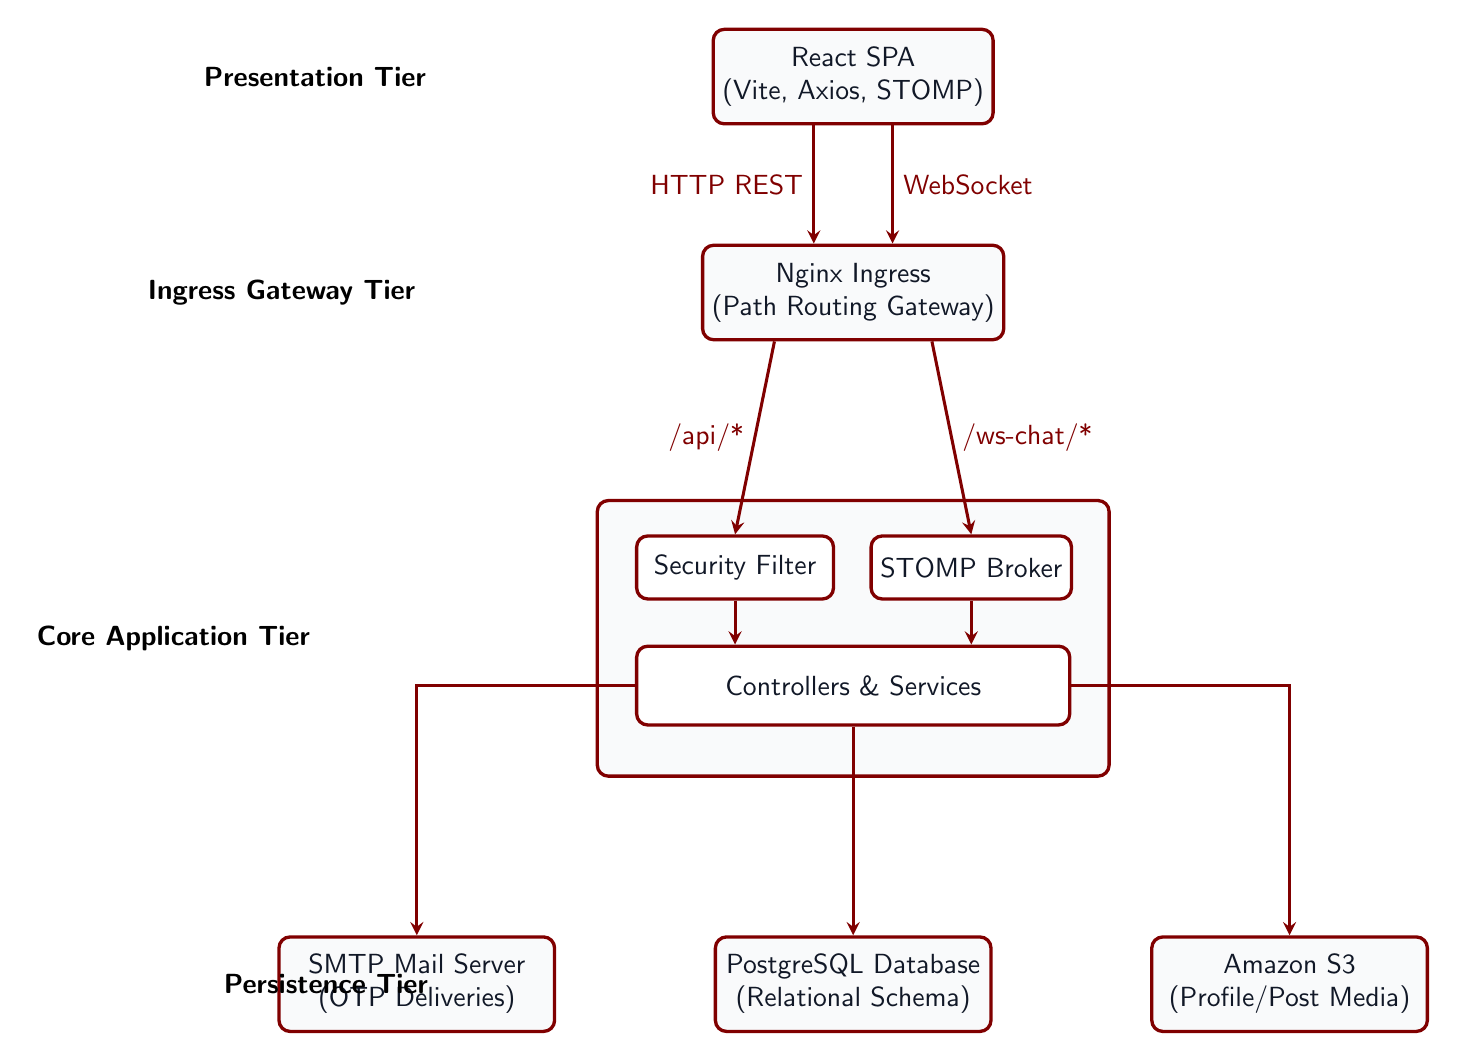
\begin{tikzpicture}[node distance=1.5cm, auto]
        % --- presentation tier ---
        \node [block, fill=LightGrey, draw=RguktMaroon] (react) {React SPA \\ (Vite, Axios, STOMP)};
        
        % --- ingress tier ---
        \node [block, below=1.5cm of react, fill=LightGrey] (ingress) {Nginx Ingress \\ (Path Routing Gateway)};
        
        % --- backend tier ---
        \node [block, below=2cm of ingress, fill=LightGrey, minimum width=6.5cm, minimum height=3.5cm] (backend) {};
        \node [block, fill=white, draw=RguktMaroon, minimum width=2.5cm, minimum height=0.8cm] at ($(backend.center) + (-1.5,0.9)$) (security) {Security Filter};
        \node [block, fill=white, draw=RguktMaroon, minimum width=2.5cm, minimum height=0.8cm] at ($(backend.center) + (1.5,0.9)$) (ws) {STOMP Broker};
        \node [block, fill=white, draw=RguktMaroon, minimum width=5.5cm, minimum height=1cm] at ($(backend.center) + (0,-0.6)$) (services) {Controllers \& Services};
        
        % --- storage tier ---
        \node [block, below=2cm of backend, fill=LightGrey] (postgres) {PostgreSQL Database \\ (Relational Schema)};
        \node [block, right=2cm of postgres, fill=LightGrey] (s3) {Amazon S3 \\ (Profile/Post Media)};
        \node [block, left=2cm of postgres, fill=LightGrey] (smtp) {SMTP Mail Server \\ (OTP Deliveries)};

        % Draw Labels for Tiers
        \node[left=3.5cm of react] (t1) {\textbf{Presentation Tier}};
        \node[left=3.5cm of ingress] (t2) {\textbf{Ingress Gateway Tier}};
        \node[left=3.5cm of backend] (t3) {\textbf{Core Application Tier}};
        \node[left=3.5cm of postgres] (t4) {\textbf{Persistence Tier}};

        % Connect Tiers
        \draw [arrow] ($(react.south) + (-0.5,0)$) -- node [left] {HTTP REST} ($(ingress.north) + (-0.5,0)$);
        \draw [arrow] ($(react.south) + (0.5,0)$) -- node [right] {WebSocket} ($(ingress.north) + (0.5,0)$);
        
        \draw [arrow] ($(ingress.south) + (-1,0)$) -- node [left] {/api/*} (security.north);
        \draw [arrow] ($(ingress.south) + (1,0)$) -- node [right] {/ws-chat/*} (ws.north);
        
        \draw [arrow] (security.south) -- (services.north -| security.south);
        \draw [arrow] (ws.south) -- (services.north -| ws.south);
        
        \draw [arrow] (services) -- (postgres);
        \draw [arrow] (services) -| (s3);
        \draw [arrow] (services) -| (smtp);
        
        % Draw backgrounds
        \begin{scope}[on background layer]
            \node at ($(backend.north west) + (0.2,-0.3)$) [anchor=north west] {\textbf{Spring Boot Application}};
        \end{scope}
    \end{tikzpicture}
    }
    \caption{RGUKT Connect Decoupled Architecture Blueprint}
    \label{fig:system_architecture}
\end{figure}

\section{Component Communication Protocols}
The application components communicate using three primary protocols:
\begin{enumerate}
    \item \textbf{HTTP/HTTPS REST (JSON):} Used for all standard request-response operations, including user registration, session logins, profile editing, post submissions, and job postings.
    \item \textbf{STOMP over WebSocket:} Used for duplex real-time communications. Rather than using raw WebSockets, the platform runs STOMP on top, providing sub-protocols for frame routing.
    \item \textbf{JDBC (Java Database Connectivity):} Used by the Spring Data JPA layer via a HikariCP connection pool to query and write to the PostgreSQL database.
    \item \textbf{AWS SDK (HTTP REST):} The backend uses the AWS SDK to communicate with Amazon S3. Profile picture uploads generate public S3 URLs that are stored back in PostgreSQL.
\end{enumerate}

\chapter{Technology Stack}
\label{ch:technology_stack}

The selection of the technology stack for RGUKT Connect was driven by considerations of security, developer productivity, execution performance, and deployment automation. This chapter outlines the software languages, frameworks, and storage systems used.

\section{Tech Stack Matrix}
Table~\ref{tab:tech_stack} details each layer of the application.

\begin{table}[H]
    \centering
    \caption{RGUKT Connect Layered Technology Stack}
    \label{tab:tech_stack}
    \begin{tabularx}{\textwidth}{l X l X}
        \toprule
        \textbf{Layer} & \textbf{Technology / Tool} & \textbf{Version} & \textbf{Primary Purpose / Rationale} \\
        \midrule
        Frontend Core & React & 19.2.5 & Component-based UI rendering with state synchronization. \\
        Frontend Build & Vite & 8.0.10 & Rapid hot module reloading and optimized ES module bundling. \\
        Styling System & Tailwind CSS & 4.2.4 & Utility-first CSS theme compilation. \\
        API Client & Axios & 1.17.0 & Promise-based HTTP client supporting request interception and custom headers. \\
        WS Client & @stomp/stompjs & 7.3.0 & WebSockets STOMP protocol abstraction client. \\
        Backend Engine & Spring Boot & 3.4.x / 4.x & Enterprise-grade application runner. \\
        Language & Java JDK & 21 & Modern features and performance improvements. \\
        ORM Layer & Hibernate / Spring JPA & Default & Automatic entity mapping and transaction management. \\
        DB Driver & PostgreSQL JDBC & 42.x & Database connectivity driver. \\
        Connection Pool & HikariCP & Default & High-speed JDBC connection pool. \\
        Database Engine & PostgreSQL & 15 / 16 & Relational database. \\
        Binary Storage & Amazon S3 & SDK v1/v2 & Secure object storage for media attachments. \\
        Mail Server & JavaMail / SMTP & Default & Relational connection for OTP deliveries. \\
        CI/CD Server & Jenkins & Latest & Automation server managing build pipelines. \\
        Orchestration & Kubernetes & 1.28+ & Orchestrator running replicated pods. \\
        \bottomrule
    \end{tabularx}
\end{table}

\section{Technical Rationale for Primary Choices}
\begin{itemize}
    \item \textbf{Java 21 \& Spring Boot:} JDK 21 introduces virtual threads and enhanced pattern matching, improving application performance. Spring Boot provides pre-built security configurations, WebSocket support, and JPA integrations out of the box, reducing boilerplate code.
    \item \textbf{PostgreSQL:} Chosen over NoSQL options because the core data model (users, connections, comments, likes) is highly relational. PostgreSQL supports transaction management and ACID properties, which are critical for preserving connection states and notification structures.
    \item \textbf{React 19 \& Vite:} React 19 improves concurrent rendering and state management. Vite replaces Webpack to compile code faster, accelerating the development cycle.
    \item \textbf{Amazon S3 for Binaries:} Storing image files directly inside a database degrades query performance. By offloading media files to S3 and saving only their generated public URLs in the database, the database remains compact.
\end{itemize}

\chapter{Application Workflows}
\label{ch:application_workflow}

This chapter details the operational workflows of RGUKT Connect, outlining the steps, endpoints, and data transformations for key processes.

\section{Registration \& OTP Verification Workflow}
Establishing a new user account requires dual verification: university email validation and OTP challenge.
\begin{enumerate}
    \item \textbf{Identity Submission:} The user enters their name, ID number, and email.
    \item \textbf{Backend Validation:} The frontend sends a request to:
    \begin{lstlisting}[language=bash]
    POST /api/auth/register/send-otp?email={email}&idNumber={idNumber}
    \end{lstlisting}
    The backend verifies the email domain is `@rgukt.ac.in`, the ID is 7 characters, and that neither the email nor the ID is already registered.
    \item \textbf{OTP Generation:} The backend generates a 6-digit OTP, saves it in an in-memory map (`registrationOtpStorage`) with a 5-minute expiry, and sends it via SMTP.
    \item \textbf{Bypass Check:} If the email starts with `test`, the system skips SMTP and sets the OTP to `123456`.
    \item \textbf{Submission:} The user submits their registration details, password, and the OTP to:
    \begin{lstlisting}[language=bash]
    POST /api/auth/register
    \end{lstlisting}
    \item \textbf{Commit Phase:} The backend validates the OTP. If valid, it hashes the password with BCrypt, saves a new `User` record, creates a default `UserDetails` entry (setting default branch to `CSE` and phone to `9876543210`), and deletes the OTP from the in-memory map.
\end{enumerate}

\section{Authentication \& JWT Lifecycle}
Logging in establishes a stateless session:
\begin{enumerate}
    \item \textbf{Credentials Submission:} The user submits their email and password to:
    \begin{lstlisting}[language=bash]
    POST /api/auth/login
    \end{lstlisting}
    \item \textbf{Credential Verification:} The backend verifies the email domain. It retrieves the user, validates the BCrypt password hash, and returns an error if authentication fails.
    \item \textbf{Token Issuance:} The system generates a JWT access token containing the user's email, ID number, and role, signed with the backend secret.
    \item \textbf{Client Cache:} The backend returns the JWT token and basic profile metadata. The React client saves this data as a JSON string in LocalStorage under the key `userSession`.
    \item \textbf{Authorized Requests:} The client includes the token in the `Authorization` header (`Bearer <token>`) for all subsequent API requests.
\end{enumerate}

\section{Job Posting \& Referral Workflow}
Posting a job opportunity requires specific role privileges:
\begin{enumerate}
    \item \textbf{Form Submission:} The user fills out the job details form.
    \item \textbf{API Request:} The client sends the payload with the authorization token to:
    \begin{lstlisting}[language=bash]
    POST /api/jobs
    \end{lstlisting}
    \item \textbf{Role Validation:} The backend extracts the user's role from the JWT. If the role is not `ALUMNI` or `ADMIN`, the backend rejects the request with an HTTP 403 status code.
    \item \textbf{DB Write:} If authorized, the backend creates a `Job` record linked to the posting user.
\end{enumerate}

\section{Connection \& Real-Time Notification Workflow}
Establishing a connection updates the network graph and triggers notifications:
\begin{enumerate}
    \item \textbf{Connection Request:} User A clicks "Connect" on User B's profile. The client sends a request to:
    \begin{lstlisting}[language=bash]
    POST /api/connections/request/{userId}
    \end{lstlisting}
    \item \textbf{Database Entry:} The backend creates a `Connection` record with a status of `PENDING`.
    \item \textbf{Notification Trigger:} The backend creates a `Notification` entry with the type \texttt{CONNECTION\_REQUEST} and the ID of the connection request.
    \item \textbf{Real-Time Push:} The backend pushes the notification over WebSockets to the recipient:
    \begin{lstlisting}[language=bash]
    /user/{recipientId}/queue/notifications
    \end{lstlisting}
    \item \textbf{Acceptance:} User B clicks "Accept". The client sends a request to:
    \begin{lstlisting}[language=bash]
    PUT /api/connections/accept/{requestId}
    \end{lstlisting}
    The backend updates the connection status to `ACCEPTED` and pushes a \texttt{CONNECTION\_ACCEPTED} notification back to User A.
\end{enumerate}

\section{Real-Time Messaging Workflow}
Private messaging uses WebSockets to support real-time delivery:
\begin{enumerate}
    \item \textbf{STOMP Handshake:} The client establishes a WebSocket connection:
    \begin{lstlisting}[language=bash]
    ws://<host>/ws-chat/websocket
    \end{lstlisting}
    A custom channel interceptor validates the JWT token in the `Authorization` header.
    \item \textbf{Subscription:} The client subscribes to:
    \begin{lstlisting}[language=bash]
    /user/queue/messages
    \end{lstlisting}
    \item \textbf{Message Dispatch:} When sending a message, the client posts the JSON payload to `/api/chat/send` via an HTTP POST request.
    \item \textbf{Persistence:} The backend saves the message to the database and checks if User B is currently online.
    \item \textbf{WebSocket Delivery:} The system pushes the message to User B:
    \begin{lstlisting}[language=bash]
    /user/{receiverId}/queue/messages
    \end{lstlisting}
\end{enumerate}

\chapter{Frontend Architecture}
\label{ch:frontend}

The frontend of RGUKT Connect is built as a single-page application (SPA) using React 19 and compiled with Vite. This chapter details the directory layout, state management architecture, navigation system, and theme configuration.

\section{Directory Structure}
The frontend source code is organized into folders to separate components, pages, and state context:
\begin{itemize}
    \item \textbf{`src/main.jsx`:} Entry point of the application. Configures Axios defaults (e.g., setting the backend base URL via `import.meta.env.VITE\_API\_URL || 'http://localhost:8000'`).
    \item \textbf{`src/App.jsx`:} Core router component. Configures the route paths, wraps the application inside context providers, and verifies session states.
    \item \textbf{`src/context/`:} Contains React Context files that handle global states:
    \begin{itemize}
        \item \textbf{`NotificationContext`:} Manages global STOMP connections, unread notification counts, and real-time alerts.
        \item \textbf{`UserContext`:} Fetches and caches the logged-in user's profile.
        \item \textbf{`HomeContext`:} Coordinates the community post feed, like actions, and comment additions.
        \item \textbf{`JobsContext`:} Manages the active job boards, filtering, and job creations.
        \item \textbf{`NetworkContext`:} Coordinates member search directories and connection invitations.
        \item \textbf{`MessagesContext`:} Handles private chat histories and real-time message streams.
        \item \textbf{`PromptContext`:} Coordinates modal warnings and confirmations.
    \end{itemize}
    \item \textbf{`src/pages/`:} Contains page views, including Landing, Login, Register, ForgotPassword, Home, Network, Jobs, Messages, and Profile.
    \item \textbf{`src/components/`:} Houses reusable UI components (e.g., Navbar, UserCard, PostCard, modals).
\end{itemize}

\section{State Synchronization \& Context Providers}
To prevent prop-drilling, global states are managed using React Context. The root node of the component tree is wrapped in the following provider hierarchy:
\begin{lstlisting}[language=xml]
<NotificationProvider session={session}>
  <PromptProvider>
    <UserProvider session={session}>
      <HomeProvider session={session} onLogout={handleLogout}>
        <JobsProvider session={session} onLogout={handleLogout}>
          <NetworkProvider session={session} onLogout={handleLogout}>
            <MessagesProvider session={session} onLogout={handleLogout}>
               <BrowserRouter> ... </BrowserRouter>
            </MessagesProvider>
          </NetworkProvider>
        </JobsProvider>
      </HomeProvider>
    </UserProvider>
  </PromptProvider>
</NotificationProvider>
\end{lstlisting}

This setup ensures that whenever the authenticated `session` transitions (e.g., on login or logout), the dependent contexts clean up their internal cache and reset their states.

\section{Routing \& Navigation}
Routes are split into public pages and protected workspaces using a custom `ProtectedRoute` wrapper. The route mappings are summarized in Table~\ref{tab:route_mappings}.

\begin{table}[H]
    \centering
    \caption{Frontend Route Mappings and Access Rules}
    \label{tab:route_mappings}
    \begin{tabularx}{\textwidth}{l l l X}
        \toprule
        \textbf{Route Path} & \textbf{Component} & \textbf{Access Level} & \textbf{Redirect Rule (If Unauthorized)} \\
        \midrule
        `/` & `Landing` & Public & None \\
        `/login` & `Login` & Public (Anonymous) & Redirect to `/home` if already authenticated \\
        `/register` & `Register` & Public (Anonymous) & Redirect to `/home` if already authenticated \\
        `/forgot-password` & `ForgotPassword` & Public (Anonymous) & Redirect to `/home` if already authenticated \\
        `/home` & `Home` & Protected (Session) & Redirect to `/login` if token missing \\
        `/network` & `Network` & Protected (Session) & Redirect to `/login` if token missing \\
        `/jobs` & `Jobs` & Protected (Session) & Redirect to `/login` if token missing \\
        `/messages` & `Messages` & Protected (Session) & Redirect to `/login` if token missing \\
        `/profile` & `Profile` & Protected (Session) & Redirect to `/login` if token missing \\
        `*` & (Fallback) & Redirect to `/` & N/A \\
        \bottomrule
    \end{tabularx}
\end{table}

\section{Design System \& Styling}
Styling uses Tailwind CSS v4.0. The layout theme is customized in `src/index.css` inside the `@theme` block. Core variables include:
\begin{itemize}
    \item \textbf{Brand Primary Color:} `--color-rgukt-maroon` set to `\#800000` (burgundy).
    \item \textbf{Brand Accent Color:} `--color-rgukt-gold` set to `\#ffd700` (yellow gold).
    \item \textbf{Background Neutral:} `--color-rgukt-slate` set to `\#f9fafb` (off-white).
    \item \textbf{Font Stack:} Google Fonts \textbf{Inter} for body content, \textbf{Outfit} for headers, and \textbf{Source Code Pro} for code blocks.
\end{itemize}
Hover states and micro-animations use Tailwind utility modifiers (`transition-all`, `hover:scale-[1.02]`, `active:scale-[0.98]`) to provide immediate visual feedback.

\chapter{Backend Architecture}
\label{ch:backend}

The backend of RGUKT Connect is built on Spring Boot, running on Java 21. This chapter details the server architecture, directory layout, request-response execution pipeline, and exception handling mechanism.

\section{Modular Components}
The backend source code is organized into packages to separate concerns:
\begin{itemize}
    \item \textbf{`com.uday.rguktconnect.controller`:} REST Controllers. They expose endpoints, handle request mapping, and validate parameters.
    \item \textbf{`com.uday.rguktconnect.service`:} Interface and implementation classes. They execute business logic, run database transaction boundaries, enforce validation constraints, and interface with external systems (such as AWS S3 and Java Mail).
    \item \textbf{`com.uday.rguktconnect.repository`:} Spring Data JPA Repositories. They define queries and database interaction boundaries.
    \item \textbf{`com.uday.rguktconnect.entity`:} Hibernate entities. They map Java objects to PostgreSQL tables.
    \item \textbf{`com.uday.rguktconnect.dto`:} Data Transfer Objects. They decoupled database schemas from API schemas.
    \item \textbf{`com.uday.rguktconnect.security`:} Custom filter chains, password encryptions, JWT utilities, and Web Security policies.
    \item \textbf{`com.uday.rguktconnect.exception`:} Global exception handlers that catch exceptions and translate them into standard JSON responses.
\end{itemize}

\section{Request-Response Execution Pipeline}
Every API request sent to the backend goes through a structured execution pipeline:
\begin{enumerate}
    \item \textbf{Filter Chain (JWT Extraction):} The request first hits the `JwtFilter` class. It extracts the `Authorization` header, validates the signature, extracts the claims (email, idNumber, role), and registers the authenticated user in the `SecurityContext`.
    \item \textbf{Security Configuration:} The request is verified against the security policy in `SecurityConfig`. If unauthorized or calling a protected resource without a session, the request is rejected with an HTTP 401/403 status code.
    \item \textbf{REST Controller Dispatch:} The request is routed to the corresponding controller method. The controller maps incoming JSON inputs to DTO objects.
    \item \textbf{Service Execution:} The controller invokes the service layer. The service layer executes business logic (e.g., checking if a user has permission to delete a resource) and updates data inside transaction boundaries.
    \item \textbf{Database Persistence:} The service invokes JPA repositories to execute database actions.
\end{enumerate}

Figure~\ref{fig:request_flow} illustrates this pipeline.

\begin{figure}[H]
    \centering
    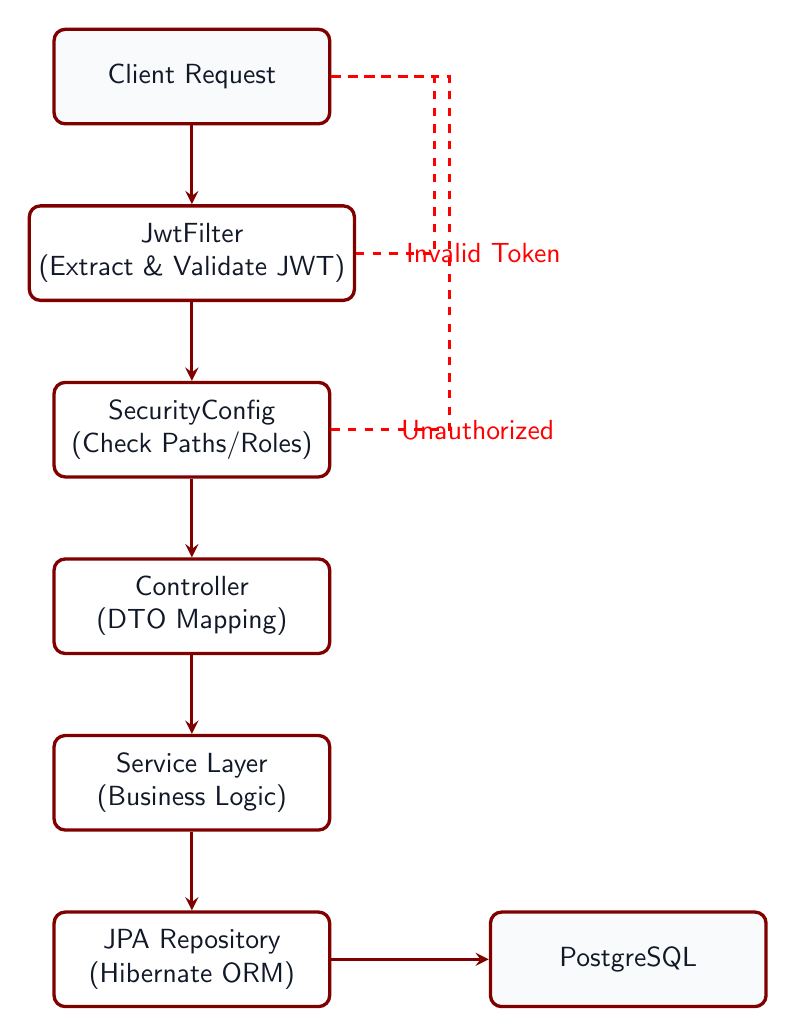
\begin{tikzpicture}[node distance=1.5cm, auto]
        \node [block, fill=LightGrey] (client) {Client Request};
        \node [block, below=1cm of client] (jwt) {JwtFilter \\ (Extract \& Validate JWT)};
        \node [block, below=1cm of jwt] (sec) {SecurityConfig \\ (Check Paths/Roles)};
        \node [block, below=1cm of sec] (ctrl) {Controller \\ (DTO Mapping)};
        \node [block, below=1cm of ctrl] (svc) {Service Layer \\ (Business Logic)};
        \node [block, below=1cm of svc] (repo) {JPA Repository \\ (Hibernate ORM)};
        \node [block, right=2cm of repo, fill=LightGrey] (db) {PostgreSQL};

        % Connect nodes
        \draw [arrow] (client) -- (jwt);
        \draw [arrow] (jwt) -- (sec);
        \draw [arrow] (sec) -- (ctrl);
        \draw [arrow] (ctrl) -- (svc);
        \draw [arrow] (svc) -- (repo);
        \draw [arrow] (repo) -- (db);

        % Error paths
        \draw [line, dashed, color=red] (jwt) -- node[right, color=red] {Invalid Token} ($(jwt.east) + (1,0)$) |- (client);
        \draw [line, dashed, color=red] (sec) -- node[right, color=red] {Unauthorized} ($(sec.east) + (1.5,0)$) |- (client);
    \end{tikzpicture}
    \caption{Backend Request-Response Pipeline and Middleware Filtering}
    \label{fig:request_flow}
\end{figure}

\section{Global Exception Handler}
To prevent server trace leakage and provide clean API responses, all uncaught exceptions are caught by `GlobalExceptionHandler`:
\begin{lstlisting}[language=java]
@RestControllerAdvice
public class GlobalExceptionHandler {
    @ExceptionHandler(RuntimeException.class)
    public ResponseEntity<?> handleRuntimeException(RuntimeException ex) {
        return ResponseEntity
                .status(HttpStatus.BAD_REQUEST) 
                .body(Map.of("error", ex.getMessage()));
    }
}
\end{lstlisting}

This advice intercepts runtime failures (such as validation failures or permission errors) and returns a JSON payload (`{"error": "<exception message>"}`) alongside a standard HTTP 400 Bad Request status code.

\chapter{Database Design \& ER Diagram}
\label{ch:database}

RGUKT Connect uses a PostgreSQL database. The schema is mapped using Hibernate ORM with the `update` DDL strategy. This chapter details the database entities, tables, relationships, and includes a detailed Entity-Relationship (ER) diagram.

\section{Database Table Definitions}
The relational database consists of ten primary tables.

\subsection{Users Table (`users`)}
Stores the core authentication and identity records.
\begin{itemize}
    \item \textbf{`id`:} `BIGINT` (Primary Key, Auto-increment).
    \item \textbf{`id\_number`:} `VARCHAR(7)` (Unique, e.g., B211449).
    \item \textbf{`name`:} `VARCHAR(255)` (Full name).
    \item \textbf{`university\_email`:} `VARCHAR(255)` (Unique, ending in `@rgukt.ac.in`).
    \item \textbf{`password`:} `VARCHAR(255)` (BCrypt hash).
    \item \textbf{`role`:} `VARCHAR(50)` (e.g., STUDENT, ALUMNI, ADMIN).
    \item \textbf{`created\_at`:} `TIMESTAMP` (Auto-generated).
\end{itemize}

\subsection{User Details Table (`user\_details`)}
Stores profile extensions. Linked to `users` via a One-to-One relationship.
\begin{itemize}
    \item \textbf{`id`:} `BIGINT` (Primary Key).
    \item \textbf{`user\_id`:} `BIGINT` (Foreign Key pointing to `users.id`, Unique).
    \item \textbf{`mobile\_number`:} `VARCHAR(15)` (Default: `9876543210`).
    \item \textbf{`personal\_email`:} `VARCHAR(255)` (Optional).
    \item \textbf{`branch`:} `VARCHAR(50)` (Academic branch, e.g., CSE, ECE).
    \item \textbf{`batch`:} `VARCHAR(10)` (e.g., 2021).
    \item \textbf{`profile\_photo`:} `VARCHAR(500)` (S3 URL).
    \item \textbf{`description`:} `TEXT` (Professional bio).
    \item \textbf{`github\_url` / `linkedin\_url`:} `VARCHAR(500)`.
    \item \textbf{`mentored\_students\_count`:} `INT` (Default: 0).
\end{itemize}

\subsection{Education Details Table (`education\_details`)}
Tracks the academic history of users. Linked via a Many-to-One relationship to `users`.
\begin{itemize}
    \item \textbf{`id`:} `BIGINT` (Primary Key).
    \item \textbf{`user\_id`:} `BIGINT` (Foreign Key pointing to `users.id`).
    \item \textbf{`institution\_name`:} `VARCHAR(255)`.
    \item \textbf{`degree`:} `VARCHAR(100)`.
    \item \textbf{`field\_of\_study`:} `VARCHAR(255)`.
    \item \textbf{`start\_year` / `end\_year`:} `INT`.
    \item \textbf{`grade`:} `VARCHAR(50)`.
\end{itemize}

\subsection{User Experiences Table (`user\_experiences`)}
Tracks the professional history of users. Linked via a Many-to-One relationship to `users`.
\begin{itemize}
    \item \textbf{`id`:} `BIGINT` (Primary Key).
    \item \textbf{`user\_id`:} `BIGINT` (Foreign Key pointing to `users.id`).
    \item \textbf{`title` / `company\_name` / `location`:} `VARCHAR(255)`.
    \item \textbf{`employment\_type` / `location\_type`:} `VARCHAR(100)` (e.g., Remote, On-site).
    \item \textbf{`start\_date` / `end\_date`:} `DATE`.
    \item \textbf{`is\_current\_role`:} `BOOLEAN`.
    \item \textbf{`description`:} `TEXT`.
\end{itemize}

\subsection{Projects Table (`projects`)}
Tracks user projects. Linked via a Many-to-One relationship to `users`.
\begin{itemize}
    \item \textbf{`id`:} `BIGINT` (Primary Key).
    \item \textbf{`user\_id`:} `BIGINT` (Foreign Key pointing to `users.id`).
    \item \textbf{`title`:} `VARCHAR(255)`.
    \item \textbf{`description`:} `TEXT`.
    \item \textbf{`project\_url` / `repo\_url`:} `VARCHAR(500)`.
\end{itemize}

\subsection{Posts Table (`posts`)}
Stores community feed items. Linked to `users` as author.
\begin{itemize}
    \item \textbf{`id`:} `BIGINT` (Primary Key).
    \item \textbf{`author\_id`:} `BIGINT` (Foreign Key pointing to `users.id`).
    \item \textbf{`type`:} `VARCHAR(50)` (e.g., text, referral, image).
    \item \textbf{`content`:} `TEXT`.
    \item \textbf{`code\_snippet`:} `TEXT` (Optional, supports code shares).
    \item \textbf{`company` / `role`:} `VARCHAR(255)` (Optional, for referral type).
    \item \textbf{`media\_url`:} `VARCHAR(500)` (AWS S3 file attachment).
    \item \textbf{`created\_at`:} `TIMESTAMP`.
\end{itemize}

\subsection{Comments Table (`comments`)}
Nested post comment structures. Linked to `posts` and `users` (as author).
\begin{itemize}
    \item \textbf{`id`:} `BIGINT` (Primary Key).
    \item \textbf{`post\_id`:} `BIGINT` (Foreign Key pointing to `posts.id`).
    \item \textbf{`author\_id`:} `BIGINT` (Foreign Key pointing to `users.id`).
    \item \textbf{`parent\_id`:} `BIGINT` (Self-referential Foreign Key pointing to `comments.id` for nested replies).
    \item \textbf{`content`:} `TEXT`.
    \item \textbf{`created\_at`:} `TIMESTAMP`.
\end{itemize}

\subsection{Connections Table (`connections`)}
Handles networking relationships. Includes a unique constraint on the pair `(sender\_id, receiver\_id)`.
\begin{itemize}
    \item \textbf{`id`:} `BIGINT` (Primary Key).
    \item \textbf{`sender\_id`:} `BIGINT` (Foreign Key pointing to `users.id`).
    \item \textbf{`receiver\_id`:} `BIGINT` (Foreign Key pointing to `users.id`).
    \item \textbf{`status`:} `VARCHAR(50)` (e.g., PENDING, ACCEPTED).
    \item \textbf{`created\_at` / `updated\_at`:} `TIMESTAMP`.
\end{itemize}

\subsection{Chat Messages Table (`chat\_messages`)}
Persistent history for chat messages.
\begin{itemize}
    \item \textbf{`id`:} `BIGINT` (Primary Key).
    \item \textbf{`sender\_id`:} `BIGINT` (Foreign Key pointing to `users.id`).
    \item \textbf{`receiver\_id`:} `BIGINT` (Foreign Key pointing to `users.id`).
    \item \textbf{`content`:} `TEXT` (Encrypted or raw text storage).
    \item \textbf{`is\_read`:} `BOOLEAN` (Default: false).
    \item \textbf{`timestamp`:} `TIMESTAMP`.
\end{itemize}

\subsection{Notifications Table (`notifications`)}
Tracks alerts.
\begin{itemize}
    \item \textbf{`id`:} `BIGINT` (Primary Key).
    \item \textbf{`recipient\_id`:} `BIGINT` (Foreign Key pointing to `users.id`).
    \item \textbf{`sender\_id`:} `BIGINT` (Foreign Key pointing to `users.id`).
    \item \textbf{`type`:} `VARCHAR(100)` (e.g., CONNECTION\_REQUEST, CONNECTION\_ACCEPTED).
    \item \textbf{`related\_id`:} `BIGINT` (Polymorphic resource ID).
    \item \textbf{`is\_read`:} `BOOLEAN`.
    \item \textbf{`created\_at`:} `TIMESTAMP`.
\end{itemize}

\section{Database ER Diagram}
Figure~\ref{fig:er_diagram} shows the database schema relationships.

\begin{figure}[H]
    \centering
    \scalebox{0.75}{
    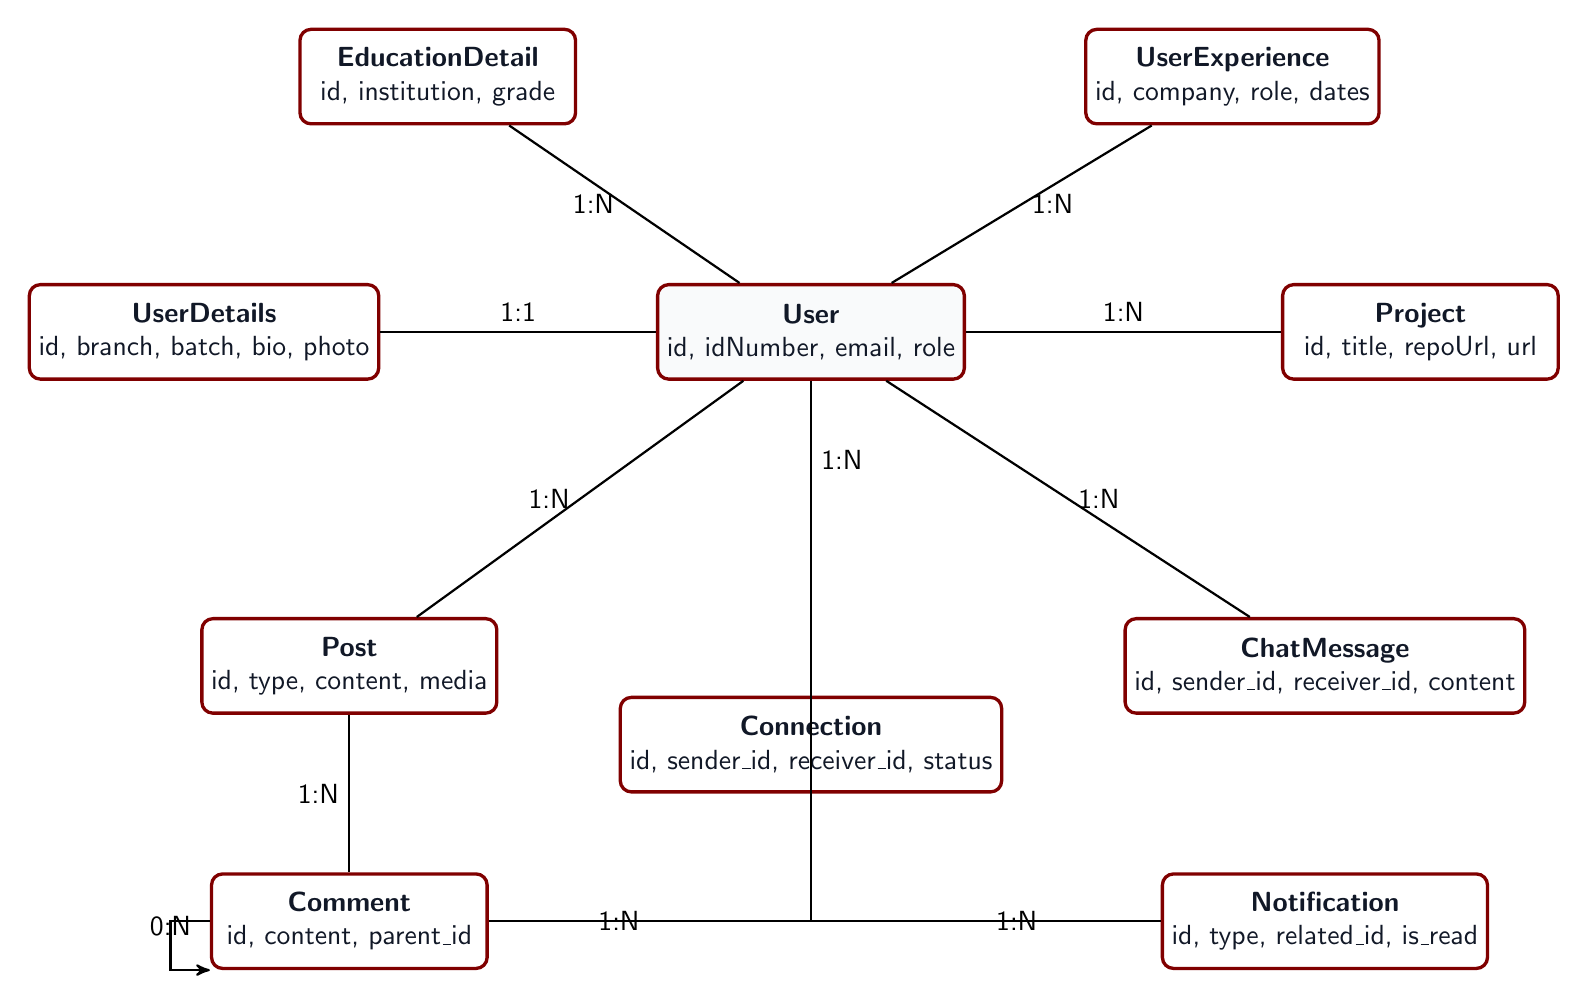
\begin{tikzpicture}[node distance=2.2cm, auto, >=stealth']
        % Entities
        \node [block, fill=LightGrey] (user) {\textbf{User} \\ id, idNumber, email, role};
        \node [block, left=3.5cm of user] (det) {\textbf{UserDetails} \\ id, branch, batch, bio, photo};
        \node [block, above left=2cm and 1cm of user] (edu) {\textbf{EducationDetail} \\ id, institution, grade};
        \node [block, above right=2cm and 1.5cm of user] (exp) {\textbf{UserExperience} \\ id, company, role, dates};
        \node [block, right=4cm of user] (proj) {\textbf{Project} \\ id, title, repoUrl, url};
        
        \node [block, below left=3cm and 2cm of user] (post) {\textbf{Post} \\ id, type, content, media};
        \node [block, below=4cm of user] (conn) {\textbf{Connection} \\ id, sender\_id, receiver\_id, status};
        \node [block, below right=3cm and 2cm of user] (msg) {\textbf{ChatMessage} \\ id, sender\_id, receiver\_id, content};
        
        \node [block, below=2cm of post] (comm) {\textbf{Comment} \\ id, content, parent\_id};
        \node [block, below=2cm of msg] (notif) {\textbf{Notification} \\ id, type, related\_id, is\_read};

        % Relationships
        % One-to-One
        \draw [thick, -] (user) -- node [above] {1:1} (det);
        
        % One-to-Many User -> sub profiles
        \draw [thick, -] (user) -- node [left] {1:N} (edu);
        \draw [thick, -] (user) -- node [right] {1:N} (exp);
        \draw [thick, -] (user) -- node [above] {1:N} (proj);
        
        % One-to-Many User -> feed & interactions
        \draw [thick, -] (user) -- node [left] {1:N} (post);
        \draw [thick, -] (user) -- node [near start, right] {1:N} (conn);
        \draw [thick, -] (user) -- node [right] {1:N} (msg);
        
        % Connections
        \draw [thick, -] (post) -- node [left] {1:N} (comm);
        \draw [thick, -] (user) |- node [near end, left] {1:N} (comm);
        \draw [thick, -] (user) |- node [near end, right] {1:N} (notif);
        
        % Self join on Comment
        \draw [thick, ->] (comm.west) -- ++(-0.5,0) |- node [above, near start] {0:N} (comm.south west);
    \end{tikzpicture}
    }
    \caption{RGUKT Connect Relational Database ER Schema Diagram}
    \label{fig:er_diagram}
\end{figure}

\chapter{API Documentation}
\label{ch:api}

RGUKT Connect exposes REST endpoints for transactional workflows and WebSocket endpoints for real-time messaging. This chapter defines the API pathways, parameters, and request/response JSON schemas.

\section{Authentication \& Session Gateway}

\subsection{Send Registration OTP}
Sends a verification OTP to the user's university email address.
\begin{itemize}
    \item \textbf{Path:} `POST /api/auth/register/send-otp`
    \item \textbf{Parameters (Query):}
    \begin{itemize}
        \item `email` (string, required): e.g., `B211449@rgukt.ac.in`
        \item `idNumber` (string, required): e.g., `B211449`
    \end{itemize}
    \item \textbf{Response:} `200 OK` on success.
\end{itemize}

\subsection{Complete Registration}
Registers a new user account after validating the email OTP.
\begin{itemize}
    \item \textbf{Path:} `POST /api/auth/register`
    \item \textbf{Request Body (JSON):}
    \begin{lstlisting}[language=json]
    {
      "idNumber": "B211449",
      "name": "Jane Doe",
      "universityEmail": "B211449@rgukt.ac.in",
      "password": "securepassword123",
      "role": "STUDENT",
      "otp": "123456"
    }
    \end{lstlisting}
    \item \textbf{Response Body (JSON - 200 OK):}
    \begin{lstlisting}[language=json]
    {
      "id": 15,
      "idNumber": "B211449",
      "name": "Jane Doe",
      "universityEmail": "B211449@rgukt.ac.in",
      "role": "STUDENT",
      "createdAt": "2026-08-18T12:00:00Z"
    }
    \end{lstlisting}
\end{itemize}

\subsection{Log In (Get JWT)}
Authenticates credentials and returns a JWT access token.
\begin{itemize}
    \item \textbf{Path:} `POST /api/auth/login`
    \item \textbf{Request Body (JSON):}
    \begin{lstlisting}[language=json]
    {
      "universityEmail": "B211449@rgukt.ac.in",
      "password": "securepassword123"
    }
    \end{lstlisting}
    \item \textbf{Response Body (JSON - 200 OK):}
    \begin{lstlisting}[language=json]
    {
      "accessToken": "eyJhbGciOiJIUzI1NiIsInR5cCI6IkpXVCJ9...",
      "user": {
        "id": 15,
        "idNumber": "B211449",
        "name": "Jane Doe",
        "universityEmail": "B211449@rgukt.ac.in",
        "role": "STUDENT",
        "createdAt": "2026-08-18T12:00:00Z"
      }
    }
    \end{lstlisting}
\end{itemize}

\section{Profile Management}

\subsection{Fetch Active User Profile}
Retrieves the profile details of the authenticated user.
\begin{itemize}
    \item \textbf{Path:} `GET /api/users/profile`
    \item \textbf{Headers:} `Authorization: Bearer <token>`
    \item \textbf{Response Body (JSON - 200 OK):}
    \begin{lstlisting}[language=json]
    {
      "id": 15,
      "idNumber": "B211449",
      "name": "Jane Doe",
      "universityEmail": "B211449@rgukt.ac.in",
      "mobileNumber": "9876543210",
      "personalEmail": "jane.doe@gmail.com",
      "branch": "CSE",
      "batch": "2021",
      "profilePhoto": "https://rgukt-connect-bucket.s3.amazonaws.com/profiles/B211449-avatar.png",
      "description": "Software engineer intern",
      "githubUrl": "https://github.com/janedoe",
      "linkedinUrl": "https://linkedin.com/in/janedoe",
      "mentoredStudentsCount": 0,
      "projects": [],
      "experiences": [],
      "education": []
    }
    \end{lstlisting}
\end{itemize}

\section{Connection \& Networking Actions}

\subsection{Request Connection}
Sends a pending connection invitation to another user.
\begin{itemize}
    \item \textbf{Path:} `POST /api/connections/request/{receiverId}`
    \item \textbf{Headers:} `Authorization: Bearer <token>`
    \item \textbf{Response:} `200 OK` (creates request and triggers WS notification).
\end{itemize}

\subsection{Accept Connection}
Accepts a pending connection request.
\begin{itemize}
    \item \textbf{Path:} `PUT /api/connections/accept/{requestId}`
    \item \textbf{Headers:} `Authorization: Bearer <token>`
    \item \textbf{Response:} `200 OK` (updates state and triggers WS notification).
\end{itemize}

\subsection{Fetch Connection Status}
Checks the connection state between the active user and a target user.
\begin{itemize}
    \item \textbf{Path:} `GET /api/connections/status/{targetUserId}`
    \item \textbf{Headers:} `Authorization: Bearer <token>`
    \item \textbf{Response Body (JSON - 200 OK):}
    \begin{lstlisting}[language=json]
    {
      "status": "PENDING_RECEIVED",
      "connectionId": 48
    }
    \end{lstlisting}
\end{itemize}

\section{Job Board Operations}

\subsection{Post Job Opportunity}
Publishes a job or internship opportunity. Requires the role `ALUMNI` or `ADMIN`.
\begin{itemize}
    \item \textbf{Path:} `POST /api/jobs`
    \item \textbf{Headers:} `Authorization: Bearer <token>`
    \item \textbf{Request Body (JSON):}
    \begin{lstlisting}[language=json]
    {
      "company": "Google",
      "role": "Systems Engineer",
      "location": "Hyderabad, India",
      "salary": "25 LPA",
      "applyUrl": "https://careers.google.com/jobs/...",
      "type": "Full-time",
      "expiresAt": "2026-10-31",
      "referralAvailable": true,
      "category": "Software Engineering"
    }
    \end{lstlisting}
    \item \textbf{Response Body (JSON - 200 OK):}
    \begin{lstlisting}[language=json]
    {
      "id": 8,
      "company": "Google",
      "role": "Systems Engineer",
      "location": "Hyderabad, India",
      "salary": "25 LPA",
      "applyUrl": "https://careers.google.com/jobs/...",
      "type": "Full-time",
      "postedBy": "Alumni John",
      "postedById": 3,
      "referralAvailable": true,
      "category": "Software Engineering",
      "createdAt": "2026-08-18T15:30:00Z",
      "expiresAt": "2026-10-31"
    }
    \end{lstlisting}
\end{itemize}

\section{WebSocket Channels}

\subsection{STOMP Endpoint}
\begin{itemize}
    \item \textbf{URL:} `ws://<host>/ws-chat/websocket`
    \item \textbf{Handshake Headers:} `Authorization: Bearer <token>`
\end{itemize}

\subsection{Subscribed Channels}
\begin{itemize}
    \item \textbf{`/user/queue/messages`:} Receives real-time private messages from connected users.
    \item \textbf{`/user/queue/notifications`:} Receives real-time connection alerts.
\end{itemize}

\chapter{Authentication Mechanics}
\label{ch:authentication}

RGUKT Connect uses stateless token-based authentication. This chapter details password hashing, JSON Web Token (JWT) signatures, request-level verification filters, and WebSocket handshake authentication.

\section{Password Hashing via BCrypt}
User passwords are encrypted before storage. The system uses Spring Security's `BCryptPasswordEncoder` with a default strength factor of 10. BCrypt incorporates a random salt for each hash, securing stored passwords against rainbow table attacks:
\begin{lstlisting}[language=java]
String securePassword = passwordEncoder.encode(requestDTO.getPassword());
user.setPassword(securePassword);
\end{lstlisting}

During login, the system matches the raw password against the stored hash using:
\begin{lstlisting}[language=java]
passwordEncoder.matches(loginRequest.getPassword(), user.getPassword())
\end{lstlisting}

\section{JWT Signature \& Payload Claims}
Upon successful authentication, the server generates a signed JWT access token. 
\begin{itemize}
    \item \textbf{Signature Algorithm:} HMAC-SHA256 (`HS256`).
    \item \textbf{Signing Key:} Loaded from the `JWT\_SECRET` environment variable.
    \item \textbf{Payload Claims:} The JWT contains:
    \begin{itemize}
        \item Subject (`sub`): University email address.
        \item Issued At (`iat`): Timestamp of creation.
        \item Expiration (`exp`): Timestamp when the token expires.
        \item Custom Claims: User ID number and account Role.
    \end{itemize}
\end{itemize}

\section{Request Filtering: `JwtFilter`}
For HTTP requests, the custom `JwtFilter` class (which extends `OncePerRequestFilter`) processes the security context:
\begin{enumerate}
    \item It extracts the `Authorization` header from the incoming request.
    \item It checks if the header begins with the prefix `Bearer `.
    \item It parses the token using the secret key and extracts the email and user roles.
    \item If the token is valid, it builds a `UsernamePasswordAuthenticationToken` and sets it in Spring Security's context:
    \begin{lstlisting}[language=java]
    SecurityContextHolder.getContext().setAuthentication(authenticationToken);
    \end{lstlisting}
\end{enumerate}

\section{WebSocket Handshake Authentication Interceptor}
Since WebSockets are upgrade connections that do not use standard HTTP filters after the initial handshake, securing STOMP frames requires a different approach.

The application registers a custom channel interceptor in `WebSocketConfig` that intercepts incoming STOMP command headers during the connection handshake (`CONNECT` frame):
\begin{enumerate}
    \item The client includes the JWT token in the `Authorization` header inside the STOMP connection headers.
    \item The `configureClientInboundChannel` interceptor extracts the `Authorization` header.
    \item It parses and validates the token.
    \item If valid, it extracts the user's details and registers a custom `Principal` object linked to the user's unique Database ID (converted to a string).
    \item This mapping allows the backend to route private messages to specific users using:
    \begin{lstlisting}[language=java]
    messagingTemplate.convertAndSendToUser(recipientId.toString(), "/queue/messages", messageDto);
    \end{lstlisting}
\end{enumerate}

\chapter{Security Architecture \& Hardening}
\label{ch:security}

This chapter reviews the security measures implemented in RGUKT Connect and outlines recommendations for future hardening.

\section{Implemented Security Controls}
\begin{itemize}
    \item \textbf{Identity Verification Restrictions:} Only users with `@rgukt.ac.in` emails can register. Student registration IDs are checked to ensure they contain exactly 7 characters, preventing external sign-ups.
    \item \textbf{In-Memory OTP Protection:} OTP codes are stored in-memory using `ConcurrentHashMap` caches with an automatic 5-minute timeout. This prevents long-term storage of temporary codes.
    \item \textbf{Stateless Authorization:} System actions require a JWT token. This eliminates session hijacking risks on the server by removing all server-side session state.
    \item \textbf{CORS Configuration:} The backend enforces CORS policies using the `CORS\_ALLOWED\_ORIGINS` environment variable. The filter checks the request origin and blocks requests from unauthorized domains.
    \item \textbf{S3 File Storage Isolation:} S3 uploads are saved using unique paths linked to user IDs and timestamps. The application does not accept custom file names, protecting the system against directory traversal attacks.
    \item \textbf{SQL Injection Prevention:} Database queries use Spring Data JPA's parameterized methods. The Hibernate engine compiles these queries into prepared statements, preventing SQL injection vulnerabilities.
\end{itemize}

\section{Future Security Recommendations}
\begin{enumerate}
    \item \textbf{SSL/TLS Encryption:} Endpoints must use HTTPS. Production deployments should configure Nginx Ingress to terminate TLS certificates (using Let's Encrypt or similar tools) to encrypt data in transit.
    \item \textbf{Rate Limiting on OTP Endpoints:} The API currently does not restrict how often a user can call `send-otp`. Attackers could exploit this to flood the SMTP queue or spam users. Implementing a rate limiter (such as Bucket4j or Redis token bucket) would prevent abuse.
    \item \textbf{JWT Blocklisting with Redis:} Because JWT tokens are stateless, they cannot be invalidated before their expiration date. Implementing a Redis-based blocklist would allow users to log out immediately or enable administrators to revoke compromised tokens.
    \item \textbf{Secrets Management:} The production environments should load database passwords, S3 keys, and JWT secrets from a secure secrets provider (such as HashiCorp Vault or Kubernetes Secrets) instead of plain text environment files.
    \item \textbf{Input Sanitization:} To protect the platform against Cross-Site Scripting (XSS) attacks in the community feed, the client and server should sanitize user input, scrubbing HTML tags and scripts from post bodies and code snippets.
\end{enumerate}

\chapter{Deployment \& Orchestration}
\label{ch:deployment}

This chapter details the deployment architecture of RGUKT Connect, covering containerization, Kubernetes orchestration, ingress routing, and the CI/CD pipeline.

\section{Dockerization (Multi-Stage Build)}
The backend uses a multi-stage Docker build to keep production images small and secure. The compiler environment (JDK) is separated from the runtime environment (JRE).

Listing~\ref{lst:dockerfile} shows the backend `Dockerfile`.

\begin{lstlisting}[language=SQL, caption=Backend Multi-Stage Dockerfile, label=lst:dockerfile]
# Stage 1: Build stage
FROM maven:3.9.9-eclipse-temurin-21 AS build
WORKDIR /app
COPY pom.xml .
RUN mvn dependency:go-offline
COPY . .
RUN mvn clean package -DskipTests

# Stage 2: Runtime stage
FROM eclipse-temurin:21-jre
WORKDIR /app
COPY --from=build /app/target/*.jar app.jar
EXPOSE 8000
ENTRYPOINT ["java","-jar","app.jar","--server.port=8000"]
\end{lstlisting}

\section{Kubernetes Orchestration}
The platform is designed to run in a Kubernetes cluster, providing horizontal scaling and self-healing.

\subsection{Deployment Controller (`deployment.yaml`)}
Manages replicas and deployment updates.
\begin{itemize}
    \item \textbf{Replicas:} 2 pods running the image `udayangari/rgukt-connect-backend:v2`.
    \item \textbf{Rolling Update Strategy:} Configured with `maxSurge: 1` and `maxUnavailable: 0`. This guarantees zero-downtime updates by spinning up a new container before stopping the old one.
    \item \textbf{Probes:}
    \begin{itemize}
        \item \textbf{Readiness Probe:} Calls HTTP `/api/auth/health` on port 8000 after a 90-second delay to check when the pod is ready to receive traffic.
        \item \textbf{Liveness Probe:} Calls HTTP `/api/auth/health` on port 8000 after a 120-second delay to monitor container health.
    \end{itemize}
    \item \textbf{Resource Allocations:}
    \begin{itemize}
        \item CPU: Request 250m, Limit 500m.
        \item Memory: Request 512Mi, Limit 1Gi.
    \end{itemize}
\end{itemize}

\subsection{Service Mapping (`service.yaml`)}
The backend pods are exposed inside the cluster using a NodePort Service:
\begin{itemize}
    \item \textbf{Service Name:} `backend-service`
    \item \textbf{Type:} `NodePort`
    \item \textbf{Ports:} Internal port 8000 mapped to NodePort 32001. This exposes the service on port 32001 across all cluster nodes.
\end{itemize}

\subsection{Ingress Router Configuration (`ingress.yaml`)}
An Nginx Ingress Controller handles external routing:
\begin{itemize}
    \item \textbf{API Routing:} Routes \texttt{/api(/|\$)(.*)} requests to \texttt{backend-service:8000}.
    \item \textbf{WebSocket Upgrade Routing:} Routes WebSocket connections on path \texttt{/ws-chat(/|\$)(.*)} directly to the backend pods to support real-time communication.
\end{itemize}

\section{Jenkins CI/CD Pipeline}
The build pipeline is automated using a Jenkins declarative pipeline (`Jenkinsfile`). The deployment process consists of ten stages:
\begin{enumerate}
    \item \textbf{Checkout:} Pulls the latest source code from the Git repository.
    \item \textbf{Verify Environment File:} Verifies the presence of the environment file `/opt/rgukt-connect/.env`.
    \item \textbf{Docker Hub Login:} Authenticates with Docker Hub using Jenkins credentials (`dockerhub-creds`).
    \item \textbf{Build Docker Image:} Compiles and packages the application inside the `backend` folder, tag-naming the resulting image.
    \item \textbf{Push Image:} Pushes the image to Docker Hub.
    \item \textbf{Stop Old Container:} Stops and removes the active container on the host machine.
    \item \textbf{Remove Old Image:} Deletes the stale container image.
    \item \textbf{Pull Latest Image:} Fetches the new build.
    \item \textbf{Run Backend:} Starts the container in the background, loading environment variables from `/opt/rgukt-connect/.env` and mapping port 8000.
    \item \textbf{Health Check:} Runs a polling loop that sends requests to `http://localhost:8000/health` up to 30 times (every 2 seconds) to confirm the server started successfully.
\end{enumerate}

\chapter{Testing \& Automated Cleanup}
\label{ch:testing}

This chapter details the testing strategies and automated test data cleanup mechanisms implemented in RGUKT Connect.

\section{Existing Test Suite}
The application contains the standard Spring Boot context initialization test:
\begin{lstlisting}[language=java]
@SpringBootTest
class RguktConnectApplicationTests {
    @Test
    void contextLoads() {
    }
}
\end{lstlisting}

This test executes during the build phase (`mvn clean package`) to verify that the application context, Spring beans, database configurations, and environment dependencies load correctly.

\section{Developer Testing Shortcuts}
To support manual testing and local development, the platform provides two developer features in the authentication layer:
\begin{enumerate}
    \item \textbf{Bypass Email Verification:} For emails starting with the prefix `test` (e.g., `teststudent@rgukt.ac.in` or `testalumni@rgukt.ac.in`), the system skips the SMTP email sending process.
    \item \textbf{Hardcoded OTP Key:} For these test accounts, the OTP is set to `123456`. This allows developers and automated scripts to register and reset passwords without access to a real email inbox.
\end{enumerate}

\section{Automated Test Data Cleanup Scheduler}
To prevent database bloating from test accounts, the system runs an automated cleanup scheduler. A background thread (`CleanupScheduler`) runs every 5 minutes (`fixedRate = 300000` milliseconds) using Spring's `@Scheduled` annotation:
\begin{itemize}
    \item \textbf{Cutoff Period:} The scheduler defines a cutoff time of exactly 2 days before the current execution time:
    \begin{lstlisting}[language=java]
    LocalDateTime cutoff = LocalDateTime.now().minusDays(2);
    \end{lstlisting}
    \item \textbf{Post Deletions:} The scheduler identifies posts created by accounts with the `test` prefix that are older than the 2-day cutoff. It deletes all nested comment replies, top-level comments, and then deletes the post entity.
    \item \textbf{Connection Deletions:} The scheduler identifies pending connection requests involving `test` accounts that are older than 2 days. It deletes associated connection request notifications and removes the connection entity.
\end{itemize}

\section{Recommended Testing Strategy}
To expand test coverage, the following testing plan is recommended:
\begin{itemize}
    \item \textbf{Unit Testing (JUnit 5 + Mockito):} Target the service layer (`UserService`, `PostService`, `ConnectionService`) to verify business rules (such as validating email domains and role permissions) using mocked database states.
    \item \textbf{Controller Integration Testing (MockMvc):} Write integration tests using `@WebMvcTest` to verify that API controllers return the correct HTTP status codes and JSON schemas.
    \item \textbf{WebSocket STOMP Testing:} Build a test client to verify that messaging frames are routed correctly over the STOMP protocol.
    \item \textbf{Frontend End-to-End (E2E) Testing:} Use Playwright or Cypress to automate user flows (such as registration, connections, and real-time chat) in a browser.
\end{itemize}

\chapter{Performance Tuning}
\label{ch:performance}

This chapter details the performance configurations implemented in RGUKT Connect and recommends tuning strategies for future scaling.

\section{Implemented Performance Configurations}
\begin{itemize}
    \item \textbf{JPA Lazy Fetching:} Entity mappings use lazy fetching (\texttt{FetchType.LAZY}) for collections (such as `likedBy` in `Post` and `likedBy` in `Comment`). This prevents the system from loading related records until they are requested.
    \item \textbf{HikariCP Connection Pool:} Database connections are managed by a HikariCP pool. HikariCP reduces connection latency by keeping a pool of active database connections open, avoiding the overhead of establishing a new TCP connection for every request.
    \item \textbf{Binary Offloading to S3:} Profile pictures and post attachments are offloaded directly to Amazon S3. The database only stores the resulting URL strings, keeping database size small and reducing query latency.
    \item \textbf{Index-Optimized Relationships:} Core tables use auto-generated indexes on primary and foreign keys, speeding up join operations.
\end{itemize}

\section{Performance Tuning Recommendations}
\begin{enumerate}
    \item \textbf{Resolve N+1 Query Issues:} When loading the community feed, the application maps each `Post` entity to a `PostResponseDTO`. This maps user details, comment counts, and like states, which can trigger additional queries for each post in the list (the N+1 query problem). Using entity graphs or fetch joins (`JOIN FETCH`) in custom JPQL queries would allow the system to load this data in a single query.
    \item \textbf{Query Pagination:} Endpoints like `GET /api/posts` and `GET /api/jobs` load all records in a single request. As the platform grows, loading all records will degrade response times. The endpoints should use Spring Data's `Pageable` interface to paginate results (e.g., loading 20 posts at a time).
    \item \textbf{API Caching with Redis:} Read-heavy endpoints that change infrequently (such as the alumni directory directory search and job board listings) should be cached using Redis. This reduces database load and speeds up response times.
    \item \textbf{Frontend Asset Optimizations:} The React client should implement code splitting using `React.lazy` and `Suspense` to load route components on demand, reducing the size of the initial JavaScript bundle.
\end{enumerate}

\chapter{Scalability Blueprint}
\label{ch:scalability}

This chapter details the architectural design and roadmap for scaling RGUKT Connect to support high user traffic and concurrent messaging.

\section{Horizontal Scaling of Backend Pods}
The Spring Boot backend is packaged as a stateless Docker container. This allows the application to be scaled horizontally by running multiple replicas in the Kubernetes cluster. Traffic is distributed across these replicas using a Kubernetes Service.

However, scaling the stateless API layer introduces challenges for features that manage state, such as WebSockets and in-memory caches.

\section{Redis Message Broker for WebSocket Sync}
Currently, the WebSocket STOMP broker is run in-memory within each backend process. If a client connects to Pod A, and another connects to Pod B, they cannot exchange messages directly because their sessions are isolated on different servers.

To support multiple backend pods, the application must use a shared message broker (such as RabbitMQ or a Redis Pub/Sub backplane) instead of the in-memory broker.

\begin{figure}[H]
    \centering
    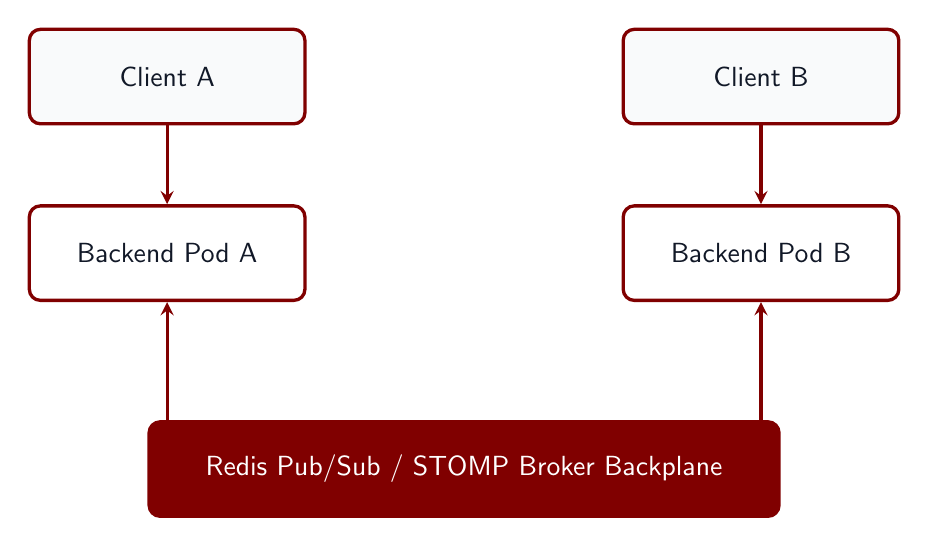
\begin{tikzpicture}[node distance=1.5cm, auto]
        \node [block, fill=LightGrey] (clientA) {Client A};
        \node [block, right=4cm of clientA, fill=LightGrey] (clientB) {Client B};
        
        \node [block, below=1cm of clientA] (podA) {Backend Pod A};
        \node [block, below=1cm of clientB] (podB) {Backend Pod B};
        
        \node [block, below=1.5cm of $(podA.south)!0.5!(podB.south)$, fill=RguktMaroon, text=white, minimum width=8cm] (redis) {Redis Pub/Sub / STOMP Broker Backplane};

        \draw [arrow] (clientA) -- (podA);
        \draw [arrow] (clientB) -- (podB);
        
        \draw [arrow, <->] (podA) -- (redis -| podA);
        \draw [arrow, <->] (podB) -- (redis -| podB);
    \end{tikzpicture}
    \caption{Distributed WebSocket Architecture using a Redis Pub/Sub Backplane}
    \label{fig:redis_pubsub}
\end{figure}

As shown in Figure~\ref{fig:redis_pubsub}, when Pod A receives a message, it publishes it to the Redis channel. Pod B, which is subscribed to the Redis channel, receives the message and forwards it to Client B, enabling cross-pod messaging.

\section{Database Scaling: Read-Write Separation}
Because user activity in social platforms is read-heavy (e.g., browsing feeds, searching directories, checking jobs), the database can become a bottleneck. The following database architecture is recommended for scaling:
\begin{itemize}
    \item \textbf{Write Master Database:} A single database instance that processes all write operations (e.g., new posts, connections, chat logs).
    \item \textbf{Read Replicas:} Multiple read-only databases synced asynchronously with the master. The application routes read operations (such as directory queries) to these replicas, distributing the database load.
\end{itemize}

\section{Content Delivery Network (CDN) Integration}
To reduce load on the origin server, static assets (such as profile images and post attachments uploaded to Amazon S3) should be served through a CDN (such as Amazon CloudFront or Cloudflare). The CDN caches these assets at edge locations close to users, reducing latency and bandwidth costs.

\chapter{Troubleshooting \& Operational Runbook}
\label{ch:troubleshooting}

This chapter details the troubleshooting steps for common operational issues encountered during development, deployment, or system executions.

\section{Database Connectivity Failures}
\begin{itemize}
    \item \textbf{Symptom:} The Spring Boot application fails to boot, throwing a `HikariPool-1 - Connection is not available` error.
    \item \textbf{Cause:} The application cannot establish a socket connection to PostgreSQL, typically due to incorrect credentials, an inactive database process, or an unmapped database URL.
    \item \textbf{Resolution:}
    \begin{enumerate}
        \item Verify that the PostgreSQL service is active:
        \begin{lstlisting}[language=bash]
        systemctl status postgresql
        \end{lstlisting}
        \item Verify that the environment variables (`DB\_URL`, `DB\_USERNAME`, `DB\_PASSWORD`) are loaded by the process.
        \item For local development, check that the database `rgukt\_connect` exists in PostgreSQL.
    \end{enumerate}
\end{itemize}

\section{CORS Policy Violations}
\begin{itemize}
    \item \textbf{Symptom:} API requests fail in the browser with the error: `Access to XMLHttpRequest has been blocked by CORS policy`.
    \item \textbf{Cause:} The client application's origin does not match the origins allowed by the backend.
    \item \textbf{Resolution:}
    \begin{enumerate}
        \item Check the `CORS\_ALLOWED\_ORIGINS` environment variable in the backend configuration.
        \item Ensure it contains the frontend origin (e.g., `http://localhost:5173` or `http://localhost:3000`) without trailing slashes.
    \end{enumerate}
\end{itemize}

\section{WebSocket Handshake dropped}
\begin{itemize}
    \item \textbf{Symptom:} The frontend STOMP client fails to connect, throwing a protocol error or returning an HTTP 401 Unauthorized status code.
    \item \textbf{Cause:} The connection handshake header is missing the authorization token, the JWT token is expired, or the ingress gateway is not configured to upgrade HTTP connections to WebSockets.
    \item \textbf{Resolution:}
    \begin{enumerate}
        \item Check that the client includes the token in the STOMP connection headers:
        \begin{lstlisting}[language={}]
        connectHeaders: { Authorization: "Bearer " + token }
        \end{lstlisting}
        \item If deploying in Kubernetes, verify that the Nginx Ingress Controller configuration permits connection upgrades by checking these headers:
        \begin{lstlisting}[language={}]
        nginx.ingress.kubernetes.io/websocket-services: "backend-service"
        \end{lstlisting}
    \end{enumerate}
\end{itemize}

\section{Amazon S3 Media Upload Failures}
\begin{itemize}
    \item \textbf{Symptom:} Uploading profile pictures or post attachments fails, and the backend logs throw an `AmazonS3Exception: Access Denied` error.
    \item \textbf{Cause:} The backend has missing or incorrect AWS credentials, or the target S3 bucket does not exist or lacks read/write permissions.
    \item \textbf{Resolution:}
    \begin{enumerate}
        \item Check the AWS environment variables: `AWS\_ACCESS\_KEY\_ID`, `AWS\_SECRET\_ACCESS\_KEY`, `AWS\_REGION`, and `AWS\_BUCKET\_NAME`.
        \item Ensure the IAM user associated with the credentials has `s3:PutObject`, `s3:GetObject`, and `s3:DeleteObject` permissions for the target bucket.
    \end{enumerate}
\end{itemize}

\chapter{System Limitations}
\label{ch:limitations}

This chapter details the current technical limitations of the RGUKT Connect platform.

\section{In-Memory OTP Cache Storage}
\begin{itemize}
    \item \textbf{Limitation:} Registration and password recovery OTPs are stored in-memory using `ConcurrentHashMap` instances.
    \item \textbf{Impact:} This design makes the authentication layer stateful. If the backend server restarts, crashes, or scales horizontally to multiple pods, users will experience validation errors when submitting OTPs, as the validation cache is tied to the memory space of a single server instance.
\end{itemize}

\section{Monolithic Database Constraints}
\begin{itemize}
    \item \textbf{Limitation:} All data (users, connections, posts, comments, notifications, chat logs) is stored in a single PostgreSQL instance.
    \item \textbf{Impact:} The database is a single point of failure (SPOF) and a potential bottleneck as query traffic scales.
\end{itemize}

\section{Single-Node WebSocket Broker}
\begin{itemize}
    \item \textbf{Limitation:} The WebSocket STOMP service uses Spring's default `SimpleBroker`, which runs in-memory within the application process.
    \item \textbf{Impact:} As discussed in the scalability blueprint (Chapter~\ref{ch:scalability}), this setup prevents the system from running multiple backend replicas in production. Messages cannot be routed between users connected to different server instances.
\end{itemize}

\section{Email Notification Gaps}
\begin{itemize}
    \item \textbf{Limitation:} The system sends email alerts (via SMTP) only for registration and password recovery OTPs.
    \item \textbf{Impact:} Important community events (such as receiving a new connection request, connection acceptances, or direct messages) only trigger in-app notifications. If a user is offline, they will not receive email notifications about these events, which can reduce active user engagement.
\end{itemize}

\section{Session Management Security}
\begin{itemize}
    \item \textbf{Limitation:} The frontend stores JWT tokens in LocalStorage (`userSession`).
    \item \textbf{Impact:} Storing sensitive session data in LocalStorage makes the application vulnerable to Cross-Site Scripting (XSS) attacks. If an attacker injects a malicious script, they can access the token and compromise the user session.
\end{itemize}

\chapter{Feature \& Architectural Roadmap}
\label{ch:roadmap}

This chapter details the feature additions and architectural improvements planned for future updates to the RGUKT Connect platform.

\section{Short-Term Milestones (1--3 Months)}
\begin{itemize}
    \item \textbf{Distributed Cache Migration:} Replace the in-memory OTP `ConcurrentHashMap` caches with a Redis instance. This will make the authentication layer stateless, allowing the backend to scale horizontally without session dropouts.
    \item \textbf{Email Notification Alerts:} Implement email notifications (via SMTP) for connection requests, connection acceptances, and private messages received while offline.
    \item \textbf{Basic Chat Search:} Add search functionality to the chat client, allowing users to query past discussions by keywords.
\end{itemize}

\section{Medium-Term Milestones (3--6 Months)}
\begin{itemize}
    \item \textbf{WebSocket Backplane Integration:} Integrate a Redis Pub/Sub backplane with Spring's STOMP broker. This enables cross-pod messaging, allowing the backend to scale horizontally across multiple instances in the Kubernetes cluster.
    \item \textbf{Mobile Application Development:} Build a mobile application using React Native or Flutter, reusing the existing REST and WebSocket APIs.
    \item \textbf{Resume Hosting:} Extend the profile dashboard to support uploading PDF resumes, saving them to AWS S3 and indexing them for recruiter searches.
\end{itemize}

\section{Long-Term Milestones (6--12 Months)}
\begin{itemize}
    \item \textbf{Multi-Tenant Architecture:} Refactor the backend to support multi-tenancy. This will allow other educational institutions to spin up their own verified connection networks on the platform.
    \item \textbf{AI-Powered Recommendation Engine:} Implement a semantic matching engine that analyzes profile data, experience history, and skills to suggest connections, mentors, and job postings.
    \item \textbf{Secure Cookie Authentication:} Replace LocalStorage-based session tokens with HTTP-only, secure, SameSite cookies to protect the application against Cross-Site Scripting (XSS) token theft.
\end{itemize}

\chapter{Developer Contribution Guide}
\label{ch:contributing}

This chapter outlines the guidelines for developers contributing to the RGUKT Connect codebase, covering branching strategies, coding standards, and deployment tests.

\section{Branching Strategy \& Workflow}
The repository uses a Git Flow branching model:
\begin{itemize}
    \item \textbf{`main`:} Production branch. Contains stable, tested releases. Direct commits to `main` are restricted.
    \item \textbf{`develop`:} Integration branch. All features and bug fixes are integrated here first.
    \item \textbf{`feature/*`:} Feature development branches. Created from `develop` and merged back via Pull Requests (PRs).
    \item \textbf{`hotfix/*`:} Urgent production fixes. Created from `main` and merged into both `main` and `develop`.
\end{itemize}

\section{Coding Standards \& Formatting}
Developers must follow consistent formatting standards across layers.

\subsection{Backend Java Code Standards}
\begin{itemize}
    \item Use standard camelCase naming for variables and methods, and PascalCase for classes.
    \item Maintain a clean separation of concerns: Controller classes must not execute business logic directly, and service classes must not interact with database JDBC layers directly.
    \item Document public API endpoints using Swagger or SpringDoc annotations.
\end{itemize}

\subsection{Frontend React Code Standards}
\begin{itemize}
    \item Write functional components using standard ES6 syntax and React Hooks.
    \item Manage local states with the `useState` hook, and use custom Context hooks for shared global state.
    \item Enforce styling rules using Tailwind CSS utility classes, and extract complex layout blocks into reusable UI components.
\end{itemize}

\section{Commit Message Conventions}
Commits should use structured, semantic prefixes:
\begin{itemize}
    \item \textbf{`feat:`} A new functional capability (e.g., `feat: integrate S3 avatar upload`).
    \item \textbf{`fix:`} A bug fix (e.g., `fix: resolve CORS header mismatch`).
    \item \textbf{`docs:`} Documentation updates (e.g., `docs: add deployment instructions`).
    \item \textbf{`refactor:`} Code refactoring that does not change functionality (e.g., `refactor: optimize JPA fetch join`).
    \item \textbf{`test:`} Adding or modifying tests (e.g., `test: add user service unit tests`).
\end{itemize}

\section{Pre-PR Checklist}
Before opening a Pull Request, developers must complete the following steps:
\begin{enumerate}
    \item Ensure the application compiles without errors:
    \begin{lstlisting}[language=bash]
    # Backend check
    mvn clean compile
    
    # Frontend check
    npm run build
    \end{lstlisting}
    \item Run all context and unit tests:
    \begin{lstlisting}[language=bash]
    mvn test
    \end{lstlisting}
    \item Verify formatting and linting:
    \begin{lstlisting}[language=bash]
    npm run lint
    \end{lstlisting}
    \item Test API endpoints using local REST clients (such as Postman or Bruno).
\end{enumerate}

\chapter{Frequently Asked Questions}
\label{ch:faq}

This chapter answers common technical and functional questions about the RGUKT Connect platform.

\section{Identity and Authentication}

\subsection{Why is registration limited to `@rgukt.ac.in` email addresses?}
Limiting registration to university-issued email domains prevents external users from signing up, protecting the platform's community focus and security.

\subsection{Can I sign up if I do not have a university email address?}
No. The platform requires a valid `@rgukt.ac.in` email to complete the registration and verification workflow.

\subsection{How long are OTP codes valid for verification?}
Both registration and password recovery OTPs are valid for exactly 5 minutes from the time they are generated.

\section{Real-Time Messaging}

\subsection{Can I message any member in the alumni directory?}
No. To prevent spam and unsolicited messages, users must first send a connection request. Private messaging is enabled only after the recipient accepts the connection request.

\subsection{Does the chat service support offline messaging?}
Yes. If a user is offline, messages are saved in the database. When the user logs back in, the client retrieves unread messages from the backend history endpoint.

\section{Technical Architecture}

\subsection{How are profile pictures and media attachments stored?}
Media files are uploaded to Amazon S3. The database only stores the resulting public S3 URL, keeping the database footprint small and improving query performance.

\subsection{Does the platform support horizontal scaling?}
The API gateway and Spring Boot backend are stateless and can scale horizontally in Kubernetes. However, the default WebSocket STOMP broker is stateful and runs in-memory, which requires a Redis Pub/Sub backplane for horizontal scaling.

\subsection{Why do my tests with email prefixes starting with `test` not send emails?}
To simplify development and automated testing, the backend skips the SMTP email sending process for emails with the prefix `test` and sets the OTP to `123456`.

\chapter{Conclusion}
\label{ch:conclusion}

RGUKT Connect addresses the professional networking gap within the Rajiv Gandhi University of Knowledge Technologies (RGUKT) community. By building a secure, closed-loop network restricted to verified students and alumni, the platform provides a trusted space for peer-to-peer mentorship, real-time collaboration, and direct job referrals.

\section{Document Summary}
This technical documentation has detailed the system's architecture and operational design:
\begin{itemize}
    \item \textbf{System Architecture:} The platform uses a decoupled split-architecture, separating the React Vite frontend from the Java Spring Boot backend.
    \item \textbf{Data Management:} Structured relational data is stored in a PostgreSQL database, while large binary files (such as profile pictures and post attachments) are offloaded to Amazon S3.
    \item \textbf{Real-Time Communication:} Instant messaging and notification deliveries use STOMP over WebSockets, secured with custom channel interceptors.
    \item \textbf{Automated Operations:} The system uses background schedulers to clean up test data and automates building and deployment using Jenkins and Kubernetes.
\end{itemize}

\section{Platform Outlook}
As the platform grows, transitioning to a stateless caching model with Redis, scaling WebSockets with a shared message broker, and implementing cookie-based session management will prepare RGUKT Connect to scale and support future university communities.


% ==========================================
% REFERENCES (Bibliography)
% ==========================================
\nocite{*}
\bibliographystyle{plain}
\bibliography{references}

\end{document}
